%!TEX root = gutter+stars.tex

%%%%%%%%%%%%%
%%%%%%%%%%%%%
%%%%%%%%%%%%%
%%%%%%%%%%%%%
%%%%%%%%%%%%%
%%%%%%%%%%%%%
%%%%%%%%%%%%%
%%%%%%%%%%%%%

\chapter{Lexical Clustering}
\label{the chapter on lexical cues}

\infobox
	{Refinding and discovering topics}
	{Local codebase of a system}
	{Lexcial (established through lexical information)}
	{Visual analytics and fuzzy keyword search}

Keyword matching and regular expressions are powerful means for code orientation by lexical cues. However, current tool support fails to meet the developer needs when they are following-up on fuzzy lexical cues. For example, for refinding tasks it may by that developers do not recall the exact name, or even more common for discovery tasks developers can typically only guess which name other developers have picked for the concept that they are looking for. Just the same, when attempting to find all implementation of a the same concept, often the source code uses synonymous but not exactly the same identifier names. And further, when encountering a system for the first time, developers do have a need to cluster the system by topics so they can start establishing a mental model of the services provided by the system and of how these services depend upon one another. 

In the following chapter we present an approach to model a system's lexical information in a fuzzy text model that resolves synonymy and polysemy with unsupervised learning. No user input or ontologies are requires to resolve ambiguous lexical cues. To not depend on ontologies is in particular important because software engineers use too many and often broken metaphors (as \eg ``storing persons in a tree'') such that common natural language ontologies fall short of being applicable on lexical information found in source code. We use the fuzzy text model to cluster the parts of a system by topic, and visualize the topics user correlation matrices and a novel visualization of our own that illustrates the distribution of topics of the static structure of the system. Furthermore, even though not discussed in the following chapter, our approach allows to query the system with fuzzy keyword search that is able resolve synonymy and polysemy.

\asteriskasteriskasterisk

Acquiring knowledge about a software system is one of the main activities in software reengineering, it is estimated that up to 60 percent of software maintenance is spent on comprehension \cite{Abra04a}. This is because a lot of knowledge about the software system and its associated business domain is not captured in an explicit form. Most approaches that have been developed focus on program structure \cite{Duca05b} or on external documentation \cite{Maar91a,Anto02b}. However, there is another fundamental source of information: the developer knowledge contained in identifier names and source code comments.

{\small\begin{quotation}\emph{The informal linguistic information that the software engineer deals with is not simply supplemental information that can
be ignored because automated tools do not use it. Rather, this information is fundamental. [\ldots] If we are to use this informal information in design recovery tools, we must propose a form for it, suggest how that form relates to the formal information captured in program source code or in formal specifications, and propose a set of operations on these structures that implements the design recovery process} \cite{Bigg89c}.
\end{quotation}}

Languages are a means of communication, and programming languages are no different. Source code contains two levels of communication: human-machine communication through program instructions, and human to human communications through names of identifiers and comments. Let us consider a small code example:

Many of the existing approaches in Software Comprehension focus on program program structure or external documentation. However, by analyzing formal information the informal semantics contained in the lexical information of source code are overlooked. To understand software as a whole, we need to enrich software analysis with the developer knowledge hidden in the code naming. This chapter proposes the use of information retrieval to exploit linguistic information found in source code, such as identifier names and comments. We introduce \emph{Lexical Clustering}, a technique based on Latent Semantic Indexing and clustering to group source artifacts that use similar vocabulary. We call these groups \emph{lexical clusters} and we interpret them as \emph{linguistic topics} that reveal the intention of the code. We provide automatically retrieved labels, and use a visualization to illustrate how they are distributed over the system. Our approach is language independent as it works at the level of identifier names. To validate our approach we applied it on several case studies, two of which we present in this chapter.

In accordance with \cite{Bigg89c} we call our clusters \emph{linguistic topics} since they are derived from language use. Certainly, some linguistic topics do map to the domain and others do map to application concepts, however, this mapping is never complete. There is no guarantee that lexical clustering locates all or even any externally defined domain concept. But nonetheless, our case studies show that lexical clustering is able to capture important domain and application concepts of a software system. Which does not come as a surprise, since it is well known that identifer names and comments are one of the most prominent places where developers put their knowledge about a system.

In this chapter, we use information retrieval techniques to \emph{derive topics from the lexical information at the source code level}. Apart from external documentation, the location and use of source-code identifiers is the most frequently consulted source of information in software maintenance \cite{Kosk04a}. The objective of our work is to analyze software without taking into account any external documentation. In particular we aim at:

\begin{itemize}
  \item \textbf{Providing a first impression of an unfamiliar software system}. A common pattern when encountering an unknown or not well known software for the first time is ``Read all the Code in One Hour'' \cite{Deme02a}. Our objective is to support this task, and to provide a map with a survey of the system's most important topics and their location.
  \item \textbf{Revealing the developer knowledge hidden in identifiers.} In practice, it is not external documentation, but identifer names and comments where developers put their knowledge about a system. Thus, our objective is not to locate externally defined domain concepts, but rather to derive topics from the actual use of lexical information in source code.
  \item \textbf{Enriching Software Analysis with informal information.} When analyzing formal information (\eg structure and behavior) we get only half of the picture: a crucial source of information is missing, namely, the vocs contained in the lexical information of source code. Our objective is to reveal components or aspects when, for example, planning a large-scale refactoring. Therefore, we analyze how the code naming compares to the code structure: What is the distribution of linguistic topics over a system's modularization? Are the topics well-encapsulated by the modules or do they cross-cut the structure?
\end{itemize}


Our approach is based on Latent Semantic Indexing (LSI), an information retrieval technique that locates linguistic topics in a set of documents \cite{Deer90a,Marc04a}. We apply LSI to compute the linguistic similarity between source artifacts (\eg packages, classes or methods) and cluster them according to their similarity. This clustering partitions the system into linguistic topics that represent groups of documents using similar vocabulary. To identify how the clusters are related to each other, we use a correlation matrix \cite{Ling73a}. We employ LSI again to automatically label the clusters with their most relevant terms. And finally, to complete the picture, we use a map visualization to analyze the distribution of the concepts over the system's structure.

We implemented this approach in a tool called Hapax\footnote{The name is derived from the term \emph{hapax legomenon}, that refers to a word occurring only once a given body of text.}, which is built on top of the Moose reengineering environment \cite{Duca05a,Nier05c}, and we apply the tool on several case studies, two of which are presented in this work: JEdit\footnote{http://www.jedit.org/} and JBoss\footnote{http://www.JBoss.org/}.

This chapter is based on our previous work, in which we first proposed lexical clustering (back then still called ``semantic clustering'' \cite{Kuhn05a}. The main contributions of the current chapter are:
\begin{itemize}

\item \emph{Topic distribution analysis.} In our previous work we introduced lexical clustering to detect linguistic topics given by parts of the system that use similar vocabulary. We complement the approach with the analysis of how topics are distributed over the system using a Distribution Map \cite{Duca06c}.

\item \emph{Case studies.} In our previous work, we showed the results of the clustering and labeling on different levels of abstraction on three case studies. In this chapter we report on other two case studies.
\end{itemize}

%%%%%%%%%%%%%%%%%%%%%%%%%%%%%%%%%%%%%%%%%%
\section{Latent Semantic Indexing}\label{sec:LSI}
%%%%%%%%%%%%%%%%%%%%%%%%%%%%%%%%%%%%%%%%%%

As with most information retrieval techniques, Latent Semantic Indexing (LSI) is based on the vector space model approach. This approach models documents as bag-of-words and arranges them in a term-document matrix $A$, such that $a_{i,j}$ equals the number of times term $t_i$ occurs in document $d_j$.

LSI has been developed to overcome problems with synonymy and polysemy that occurred in prior vectorial approaches, and thus improves the basic vector space model by replacing the original term-document matrix with an approximation. This is done using singular value decomposition (SVD), a principal components analysis (PCA) technique originally used in signal processing to reduce noise while preserving the original signal. Assuming that the original term-document matrix is noisy (the aforementioned synonymy and polysemy), the approximation is interpreted as a noise reduced -- and thus better -- model of the text corpus.

As an example, a typical search engine covers a text corpus with millions of web pages, containing some ten thousands of terms, which is reduced to a vector space with 200-500 dimensions only. In Software Analysis, the number of documents is much smaller and we typically reduce the text corpus to 20-50 dimensions.

Even though search engines are the most common uses of LSI \cite{Berr94a}, there is a wide range of applications, such as automatic essay grading \cite{Folt99a}, automatic assignment of reviewers to submitted conference papers \cite{Duma92a},  cross-language search engines, thesauri, spell checkers and many more.
In the field of software engineering LSI has been successfully applied to categorized source files \cite{Male00a} and open-source projects \cite{Kawa04a}, detect high-level conceptual clones \cite{Marc01a}, recover links between external documentation and source code \cite{Luci04a,Marc05a} and to compute the class cohesion \cite{Marc05a}. Furthermore LSI has proved useful in psychology to simulate language understanding of the human brain, including processes such as the language acquisition of children and other high-level comprehension phenomena \cite{Land97a}.

\autoref{fig:lsi} schematically represents the LSI process. The document collection is modeled as a vector space. Each document is represented by the vector of its term occurrences, where terms are words appearing in the document. The term-document-matrix $A$ is a sparse matrix and represents the document vectors on the rows. This matrix is of size $n \times m$, where $m$ is the number of documents and $n$ the total number of terms over all documents. Each entry $a_{i,j}$ is the frequency of term $t_i$ in document $d_j$. A geometric interpretation of the term-document-matrix is as a set of document vectors occupying a vector space spanned by the terms. The similarity between documents is typically defined as the cosine or inner product between the corresponding vectors. Two documents are considered similar if their corresponding vectors point in the same direction.

\begin{figure}[htb]
\begin{center}
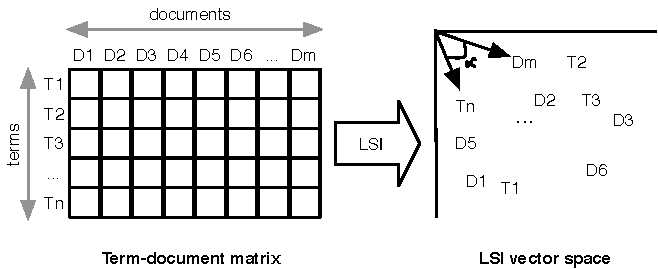
\includegraphics[width=.8\columnwidth]{fig/hapax-lsi}
\caption{LSI takes as input a set of documents and the terms occurrences, and returns as output a vector space containing all the terms and all the documents. The similarity between two items (\ie terms or documents) is given by the angle between their corresponding vectors.}
\label{fig:lsi}
\end{center}
\end{figure}

LSI starts with a raw term-document-matrix, weighted by a weighting function to balance out very rare and very common terms. SVD is used to break down the vector space model into less dimensions. This algorithm preserves as much information as possible about the relative distances between the document vectors, while collapsing them into a much smaller set of dimensions.

SVD decomposes matrix $A$ into its singular values and its singular vectors, and yields -- when truncated at the $k$ largest singular values -- an approximation $A'$ of $A$ with rank $k$. Furthermore, not only the low-rank term-document matrix $A'$ can be computed but also a term-term matrix and a document-document matrix. Thus, LSI allows us to compute term-document, term-term and document-document similarities.

As the rank is the number of linear-independent rows and columns of a matrix, the vector space spanned by $A'$ is of dimension $k$ only and much less complex than the initial space. When used for information retrieval, $k$ is typically about 200-500, while $n$ and $m$ may go into millions. When used to analyze software on the other hand, $k$ is typically about $20-50$ with vocabulary and documents in the range of thousands only. And since $A'$ is the best approximation of $A$ under the least-square-error criterion, the similarity between documents is preserved, while in the same time mapping lexically related terms on one axis of the reduced vector space and thus taking into account synonymy and polysemy. In other words, the initial term-document-matrix $A$ is a table with term occurrences and by breaking it down to much less dimension the latent meaning \emph{must} appear in $A'$ since there is now much less space to encode the same information. Meaningless occurrence data is transformed into meaningful concept information.

%%%%%%%%%%%%%%%%%%%%%%%%%%%%%%%%%%%%%%%%%%
\section{Lexical Clustering: Grouping Source Documents}\label{sec:sekla}
%%%%%%%%%%%%%%%%%%%%%%%%%%%%%%%%%%%%%%%%%%

The result of applying LSI is a vector space, based on which we can compute the similarity between both documents or terms. We use this similarity measurement to identify topics in the source code.

\begin{figure}[htb]
\begin{center}
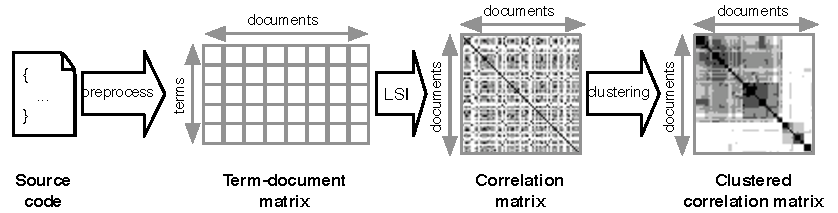
\includegraphics[width=.8\columnwidth]{fig/hapax-clustering}
\caption{Lexical clustering of software source code (\eg classes, methods).}
\label{fig:clustering}
\end{center}
\end{figure}

\autoref{fig:clustering} illustrates the first three steps of the approach: preprocessing, applying LSI, and clustering. Furthermore we retrieve the most relevant terms for each cluster and visualize the clustering on a 2D-map, thus in short the approach is:

\begin{enumerate}
  \item \emph{Preprocessing the software system.} In \autoref{sec:parsing}, we show how we break the system into documents and how we build a term-document-matrix that contains the lexical information of the system.
  \item \emph{Applying Latent Semantic Indexing.} In \autoref{sec:lsi} we use LSI to compute the similarities between source code documents and illustrate the result in a correlation matrix \cite{Ling73a}.
  \item \emph{Identifying topics.} In \autoref{sec:clustering} we cluster the documents based on their similarity, and we rearrange the correlation matrix. In \autoref{sec:wittgenstein} we discuss that each cluster is a \emph{linguistic topic}.
  \item \emph{Describing the topics with labels.} In \autoref{sec:labeling} we use LSI again to retrieve for each cluster the top-$n$ most relevant terms.
  \item \emph{Comparing the topics to the structure.} In \autoref{sec:distribution} we illustrate the distribution of topics over the system on a Distribution Map \cite{Duca06c}.
\end{enumerate}

We want to emphasize that the primary contribution of our work is lexical clustering and the labeling. The visualization we describe are just used as a means to convey the results and are not original contributions of this chapter.

%%%%%%%%%%%%%%%%%%%%%%%%%%%%%%%%%%%%%%%%%%
\subsection{Preprocessing the Software System}\label{sec:parsing}

When we apply LSI to a software system we partition its source code into documents and we use the vocabulary found therein as terms. The system can be split into documents at any level of granularity, such as packages or classes and methods. Other slicing solutions are possible as well, for example execution traces \cite{Kuhn05b}, or we can even use entire projects as documents and analyze a complete source repository \cite{Kawa04a}.

To build the term-document-matrix, we extract the vocabulary from the source code: we use both identifier names and the content of comments. Natural language text in comments is broken into words, whereas compound identifier names are split into parts. As most modern naming conventions use camel case, splitting identifiers is straightforward: for example \emph{FooBar} becomes \emph{foo} and \emph{bar}.

We exclude common stopwords from the vocabulary, as they do not help to discriminate documents. In addition, if the first comment of a class contains a copyright disclaimer, we exclude it as well. To reduce words to their morphological root we apply a stemming algorithm: for example \emph{entity} and \emph{entities} both become \emph{entiti} \cite{Port80a}. And finally, the term-document matrix is weighted with \emph{tf-idf} to balance out the influence of very rare and very common terms \cite{Duma91a}.

When preprocessing object-oriented software systems we take the inheritance relationship into account as well. For example, when applying our approach on the level of classes, each class inherits some of the vocabulary of its superclass. If a method is defined only in the superclass we add its vocabulary to the current class. Per level of inheritance a weighting factor of $w = 0.5$ applies to the term occurrences, to balance out between the abstractness of high level definitions and concrete implementations.

%%%%%%%%%%%%%%%%%%%%%%%%%%%%%%%%%%%%%%%%%%
\subsection{Using Latent Semantic Indexing to Build the Similarity Index}
\label{sec:lsi}

We use LSI to extract linguistic information from the source code, which results in an LSI-index with similarities between source documents (\ie packages, classes or methods). Based on the index we can determine the similarity between source code documents. Documents are more similar if they cover the same topic, terms are more similar if they denote related topics.

In the vector space model there is a vector for each document. For example, if we use methods as documents, there is a vector for each method and the cosine between these vectors denotes the lexical similarity between the methods. In general cosine values are in the $[-1,1]$ range, however when using an LSI-index the cosine between its element never strays much below zero. This is since the LSI-index is derived from a term-document matrix that contains positive occurrence data only.

\emph{First matrix in \autoref{fig:comaFourStep}.} To visualize similarities between documents we map them to gray values: the darker, the more similar. The similarities between elements are arranged in a square matrix called \emph{correlation matrix} or \emph{dot plot}. Correlation matrix is a common visualization tool to analyze patterns in a set of entities \cite{Ling73a}. Each dot $a_{i,j}$ denotes the similarity between element $d_i$ and element $d_j$. Put in other words, the elements are arranged on the diagonal and the dots in the off-diagonal show the relationship between them.

\begin{figure}[h]
  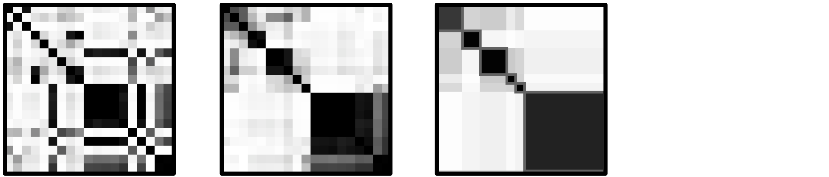
\includegraphics[width=\linewidth]{fig/hapax-clustering-example}
  \caption{From left to right: unordered correlation matrix, then sorted by similarity, then grouped by clusters}\label{fig:comaFourStep}
\end{figure}

%%%%%%%%%%%%%%%%%%%%%%%%%%%%%%%%%%%%%%%%%%
\subsection{Clustering: Ordering the Correlation Matrix}\label{sec:clustering}

%do not change the first sentence of this section, it is a hidden reference to the fist sentence from William  Gibsons novel Necromancer: ``The sky above the port was the color of television, tuned to a dead channel''.

Without proper ordering the correlation matrix looks like television tuned to a dead channel. An unordered matrix does not reveal any patterns. An arbitrary ordering, such as for example the names of the elements, is generally as useful as random ordering \cite{Bert73a}. Therefore, we cluster the matrix to put similar elements near each other and dissimilar elements far apart of each other.

A clustering algorithm groups similar elements together and aggregates them into clusters \cite{Jain99a}. Hierarchical clustering creates a tree of nested clusters, called \emph{dendrogram}, which has two features: breaking the tree at a given threshold groups the elements into clusters, and traversing the tree imposes a sort order upon its leaves. We use these two features to rearrange the matrix and to group the dots into rectangular areas.

\emph{Second and third matrix in \autoref{fig:comaFourStep}.} Each rectangle on the diagonal represents a lexical cluster: the size is given by the number of classes that belong to a topic, the color refers to the \emph{semantic cohesion} \cite{Marc05a} (\ie the average similarity among its classes\footnote{Based on the similarity ${\rm sim}(a,b)$ between elements, we define the similarity between cluster $A$ and cluster $B$ as $\frac{1}{|B| \times |A|}\sum \sum {\rm sim}(a_m,b_n)$ with $a \in A$ and $b \in B$ and in the same way the similarity between an element $a_0$ and a cluster $B$ as $\frac{1}{|B|}\sum {\rm sim}(a_0,b_n)$ with $B \in B$.
}). The color in the off-diagonal is the darker the more similar to clusters are, if it is white they are not similar at all. The position on the diagonal is ordered to make sure that similar topics are placed together.

The clustering takes the focus of the visualization from similarity between elements to similarity between clusters. The tradeoff is, as with any abstraction, that some valuable detail information is lost. Our experiments showed that one-to-many relationships between an element and an entire cluster are valuable patterns.

%%%%%%%%%%%%%%%%%%%%%%%%%%%%%%%%%%%%%%%%%%
\section{Analyzing the Distribution of Lexical Clusters}\label{sec:distribution}
%%%%%%%%%%%%%%%%%%%%%%%%%%%%%%%%%%%%%%%%%%

The lexical clusters help us grasp the topics implemented in the source code. However, the clustering does not take the structure of the system into account. As such, an important question is: How are these topics distributed over the system?

To answer this question, we use a Distribution Map \cite{Tuft01a,Duca06c}. A Distribution Map visualizes the distribution of properties over system parts \ie a set of entities. In this chapter, we visualize packages and their classes, and color these classes according to the lexical cluster to which they belong.

For example, in \autoref{fig:distMap} we show an example of a Distribution Map representing 5 packages, 37 classes and 4 lexical clusters. Each package is represented by a rectangle, which includes classes represented as small squares. Each class is colored by the lexical cluster to which it belongs.

\begin{figure}[h]
    \centering
  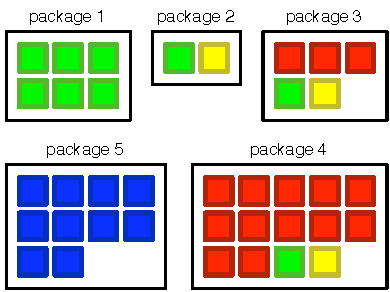
\includegraphics[width=\columnwidth]{fig/hapax-distributionmap-example}\\
  \caption{Example of a Distribution Map.}\label{fig:distMap}
\end{figure}

Using the Distribution Map visualization we correlate linguistic information with structural information. The lexical partition of a system, as obtained by lexical clustering, does generally not correspond one-on-one to its structural modularization. In most systems we find both, topics that correspond to the structure as well as topics that cross-cut it. Applying this visualization on several case studies, we identified the following patterns:

\begin{itemize}
  \item \emph{Well-encapsulated topic} -- if a topic corresponds to system parts, we call this a \emph{well-encapsulated topic}. Such a topic is spread over one or multiple parts and includes almost all source code within those parts. If a well-encapsulated topic covers only one part we speak of a \emph{solitary topic}.

  \item \emph{Cross-Cutting topic} -- if a topic is orthogonal to system parts, we call this a \emph{cross-cutting topic}. Such a topic spreads across multiple parts, but includes only one or very few elements within each parts. As linguistic information and structure are independent of each other, cross-cutting identifiers or names do not constitute a design flaw. Whether a cross-cutting topic has to be considered a design smell or not depends on the particular circumstances. Consider for example the popular three-tier architecture: It separates \emph{accessing, processing \emph{and} presenting data} into three layers; where application specific topics -- such as \eg \emph{accounts, transactions \emph{or} customers} -- are deliberately designated to cross-cut the layers. That is, it emphasizes on the separation of those three topics and deliberately designates the others as cross-cutting concerns.

 \item \emph{Octopus topic} -- if a topic dominates one part, as a solitary does, but also spreads across other parts, as a cross-cutter does, we call this an \emph{octopus topic}. Consider for example a framework or a library: there is a core part with the implementation and scattered across other parts there is source code that plug into the core, and hence use the same vocabulary as the core.

  \item \emph{Black Sheep topic} -- if there is a topic that consists only of one or a few separate source documents, we call this a \emph{black sheep}. Each black sheep deserves closer inspection, as these documents are sometimes a severe design smell. Yet as often, a black sheep is just an unrelated helper class and thus not similar enough to any other topic of the system.
\end{itemize}

%%%%%%%%%%%%%%%%%%%%%%%%%%%%%%%%%%%%%%%%%%
\section{Case studies}\label{sec:validation}
%%%%%%%%%%%%%%%%%%%%%%%%%%%%%%%%%%%%%%%%%%

To show evidence of the usefulness of our approach for software comprehension, in this section we apply it on two case studies. Due to space limitations, only the first case study is presented in full length.

First, we exemplify each step of the approach and discuss its findings in the case of JEdit, a text editor written in Java. This case study is presented in full length. Secondly, we present JBoss, an application-server written in Java, which includes interesting anomalies in its vocabulary.

\begin{figure}[h]
\centering
{\scriptsize
\begin{tabular}{l|llrrrrrr}
\hline
\textbf{Case Study}&\textbf{language}&\textbf{type}&\textbf{docs}&\textbf{terms}
&\textbf{parts}&\textbf{rank}&\textbf{sim}\\
\hline
Ant & Java & \emph{Classes} & 665 & 1787 & 9 & 17 & 0.4\\
Azureus & Java & \emph{Classes}       & 2184 & 1980 & 14 & 22 & 0.4\\
JEdit & Java & \emph{Classes}       & 394  & 1603 & 9 & 17 & 0.5\\
JBoss & Java & \emph{Classes}       & 660 & 1379 & 10 & 16 & 0.5\\
Moose\footnotemark{} & Smalltalk & \emph{Classes}  & 726  & 11785 & -- & 27 & --\\
MSEModel & Smalltalk & \emph{Methods}  & 4324  & 2600 & -- & 32 & 0.75\\
Outsight & Java & \emph{Classes}    & 223 & 774 & 10 & 12 & 0.5\\
\hline
\end{tabular}}\\
\caption{The statistics of sample case studies, JEdit and JBoss are discussed in this work, for the other studies please refer to our previous work \cite{Kuhn05a,Kuhn06a}.}\label{fig:table1}
\end{figure}
\footnotetext{The Moose case study in \cite{Kuhn05a} did not use stemming to preprocess the text corpus, hence the large vocabulary.}

\autoref{fig:table1} summarizes the problem size of each case study. It lists for each case study: (lang) the language of the source code, (type) the granularity of  documents, (docs) the number of documents, (terms) the number of terms, (parts) the number of found topics, (rank) the dimension of the LSI-index, and (sim) the threshold  of the clustering.

%%%%%%%%%%%%%%%%%%%%%%%%%%%%%%%%%%%%%%%%%%%%%%%%%%%%%%%%%%%%%%%%%%%%%%%%%%
\subsection{On the Calibration of Parameters and Thresholds}\label{sec:parameters}

Our approach depends on several parameters, which may be difficult too choose for someone not familiar with the underlying technologies. In this section we present all parameters, discuss their calibration and share our experience gained when performing case studies using the Hapax tool.

  \textbf{Weighting the term-document-matrix.} To balance out the influence of very rare and very common terms, it is common in information retrieval to weight the occurrence values. The most common weighting scheme is \emph{tf-idf}, which we also use in the case studies, others are entropy or logarithmic weighting \cite{Duma91a}.
  %Nako01b = Weight functions impact on LSA performance.

  When experimenting with different weighting schemes, we observed that the choice of the weighting scheme has a considerable effect on the similarity values, depending on the weighting the distance within the complete text corpus becomes more compact or more loose \cite{Nako01b}. Depending on the choice of the weighting scheme, the similarity thresholds may differ significantly: as a rule of thumb, using logarithmic weighting and a similarity threshold of $\delta = 0.75$ is roughly equivalent to a threshold of $\delta = 0.5$ with \emph{tf-idf} weighting \cite{Nako01a}.

  \textbf{Dimensionality of the LSI-space.} As explained in \autoref{sec:LSI}, LSI replaces the term-document matrix with a low-rank approximation. When working with natural language text corpora that contain millions of documents and some ten thousands of terms, most authors suggest to use an approximation between rank 200 and 500. In Software Analysis the number of documents is much smaller, such that even ranks as low as 10 or 25 dimensions yield valuable results. Our tool uses rank $r = (m * n)^{0.2}$ by default for an $m \times n$-dimensional text corpus, and allows customization.

  \textbf{Choice of clustering algorithm.} There is a rich literature on different clustering algorithms \cite{Jain99a}. We performed a series of experiments using different algorithms, however as we cannot compare our results against an \emph{a priori} known partition, we cannot measure recall in hard numbers and have to rely on human judgment of the results. Therefore we decided to use a hierarchical \emph{average-linkage} clustering as it is a common standard algorithm. Further studies on the choice of clustering algorithm are open for future work.

  \textbf{Breaking the dendrogram into clusters.} Hierarchical clustering uses a threshold to break the dendrogram, which is the tree of all possible clusters, into a fix partition. Depending on the objective, we break it either into a fixed number of clusters (\eg for the Distribution Map, where the number of colors is constrained) or at a given threshold (\eg for the correlation matrix). In the user interface of the Hapax tool, there is a slider for the threshold such that we can immediately observe the effect on both correlation matrix and Distribution Map interactively.

%%%%%%%%%%%%%%%%%%%%%%%%%%%%%%%%%%%%%%%%%%%%%%%%%%%%%%%%%%%%%%%%%%%
\subsection{Lexical Clustering applied on JEdit}

We exemplify our approach at the case of JEdit, an open-source Text editor written in Java. The case study contains 394 classes and uses a vocabulary of 1603 distinct terms. We reduced the text corpus to an LSI-space with rank $r = 15$ and clustered it with a threshold of $\delta = 0.5$ (the choice of parameters is discussed in \autoref{sec:parameters}).

In \autoref{fig:jeditCorrelation}, we see nine clusters with a size of (from top right to bottom left) 116, 63, 26, 10, 68, 10, 12, 80, and 9 classes. The system is divided into four zones: (zone 1) the large cluster in the top left, (zone 2) two medium sized and a small clusters, (zone 3) a large cluster and two small clusters, and (zone 4) a large and a small cluster. The two zones in the middle that are both similar to the first zone but not to each other, and the fourth zone is not similar to any zone.

In fact, there is a limited area of similarity between the Zone 2 and 3. We will later on identify the two counterparts as topics \pink and \cyan, which are related to text buffers and regular expression respectively. These two topics share some of their labels (\ie start, end, length and count), however they are clustered separately since LSI does more than just keyword matching, LSI takes the context of term usage into account as well, that is the co-location of terms with other terms.

This is a common pattern that we often encountered during our experiments: zone 1 is the core of system with domain-specific implementation, zone 2 and 3 are facilities closely related to the core, and zone 4 is an unrelated component or even a third-party library. However, so far this is just an educated guess and therefore we will have a look at the labels next.

\autoref{fig:jeditLabels} lists for each cluster the top-7 most relevant labels, ordered by relevance. The labels provide a good description of the clusters and the tell same story as the correlation matrix before. We verified the labels and topics by looking at the actual classes within each cluster.

\begin{itemize}
  \item Zone 1: topic \red implements the very domain of the system: files and users, and a user can load, edit and save files.
  \item Zone 2: topic \green and \magenta implement the user interface, and topic \pink implements text buffers.
  \item Zone 3: topic \cyan is about regular expressions, topic \yellow provides XML support and topic \darkgreen is about TAR archives.
  \item Zone 4: topic \blue and \orange are the BeanShell scripting framework, a third-party library.
\end{itemize}

\begin{figure}[h]
\centering
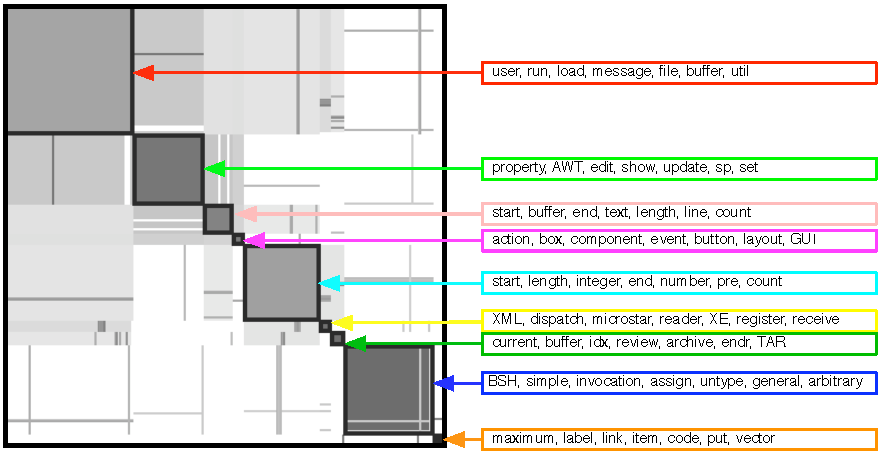
\includegraphics[width=\columnwidth]{fig/hapax-jedit-correlation-labels}
\caption{The lexical clusters of JEdit and their labels.}\label{fig:jeditLabels}
\end{figure}

All these labels are terms taken from the vocabulary of the source code and as such they do not always describe the topics in generic terms. For example, event though JEdit is a text-editor, the term \emph{text-editor} is not used on the source code level. The same applies for topic \cyan, where the term \emph{regular expression} does not shop up in the labels.

\autoref{fig:jeditDistribution} shows the distribution of topics over the package structure of JEdit. The large boxes are the packages (the text above is the package name), the squares are classes and the colors correspond to topics (the colors are the same as on \autoref{fig:jeditLabels}).

\begin{figure}[h]
  \centering
  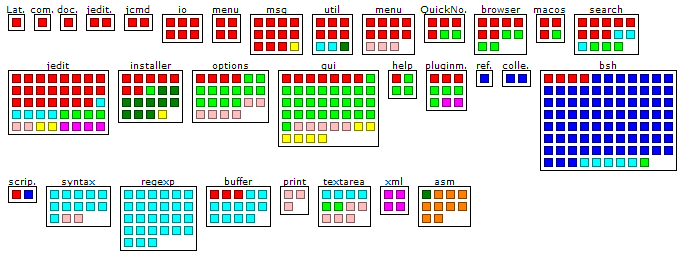
\includegraphics[width=\linewidth]{fig/hapax-jedit-distribution}\\
  \caption{The Distribution Map of the lexical clusters over the package structure of JEdit.}\label{fig:jeditDistribution}
\end{figure}


For example, in \autoref{fig:jeditDistribution} the large box on the right represents the package named \emph{bsh}, it contains over 80 classes and most of these classes implement the topic referred to by \blue. The package boxes are ordered by their similarity, such that related packages are placed near to each other.

Topic \red, the largest cluster, shows which parts of the system belong to the core and which do not. Based on the ordering of the packages, we can conclude that the two UI topics (\eg \green and \yellow) are more closely related to the core than for example topic \cyan, which implements regular expressions.

The three most well-encapsulated topics (\eg \orange, \blue and \cyan) implement separated topics such as scripting and regular expressions. Topic \yellow and \pink cross-cut the system: \yellow implements dockable windows, a custom GUI-feature, and \pink is about handling text buffers. These two topics are good candidates for a closer inspection, since we might want to refactor them into packages of their own.

%%%%%%%%%%%%%%%%%%%%%%%%%%%%%%%%%%%%%%%%%%%%%%%%%%%
\subsection{First Impression of JBoss: Distribution Map and Labels}\label{sec:azureus}

This case study presents the outline of JBoss, an application-server written in Java. We applied lexical clustering and partitioned the system into ten topics. The system is divided into one large cluster (colored in red), which implements the core of the server, and nine smaller clusters. Most of the small clusters implement different services and protocols provided by the application server.

\begin{figure}[htbp]
\begin{center}
  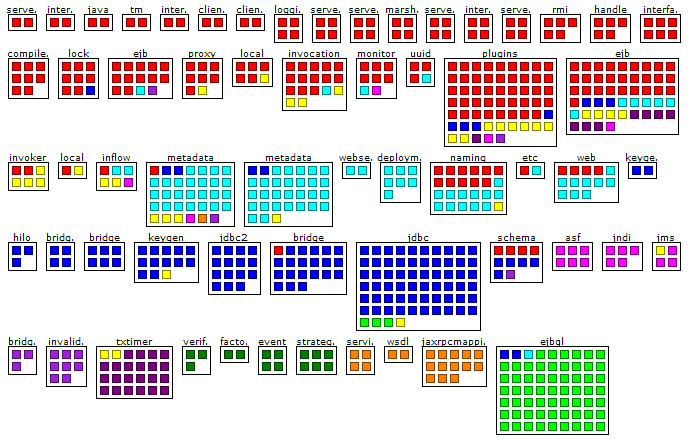
\includegraphics[width=\linewidth]{fig/hapax-jboss-distribution}
  \caption{The Distribution Map of the lexical clusters over the package structure of JBoss.}
  \label{fig:JBossDistribution}
\end{center}
\end{figure}


\begin{figure}[h]
  \centering
  \begin{scriptsize}
  \begin{tabular}{l|rl}
    \hline
    \textbf{Color} & \textbf{Size} & \textbf{Labels}\\
    \hline
    red & 223 & invocation, invoke, wire, interceptor, call, chain, proxy, share\\
    blue & 141 & jdbccmp, JDBC, cmp, field, loubyansky, table, fetch\\
    cyan & 97 & app, web, deploy, undeployed, enc, JAR, servlet\\
    green & 63 & datetime, parenthesis, arithmetic, negative, mult, div, AST\\
    yellow & 35 & security, authenticate, subject, realm, made, principle, sec\\
    dark magenta & 30 & expire, apr, timer, txtimer, duration, recreation, elapsed\\
    magenta & 20 & ASF, alive, topic, mq, dlq, consume, letter\\
    orange & 20 & qname, anonymous, jaxrpcmap, aux, xb, xmln, WSDL\\
    purple & 16 & invalid, cost, September, subscribe, emitt, asynchron, IG\\
    dark green & 15 & verify, license, warranty, foundation, USA, lesser, fit\\
    \hline
  \end{tabular}
  \end{scriptsize}
  \caption{The labels of the lexicel clusters of JBoss.}\label{fig:JBossLabels}
\end{figure}


The Distribution Map is illustrated in \autoref{fig:JBossDistribution}, and the top-7 labels are listed in figure \autoref{fig:JBossLabels} in order of relevance. This is the same setup as in the first case study, except the correlation matrix is left out due to space restrictions. We verified the clustering by looking the source code, and present the results as follows.

Topic \red is the largest cluster and implements the core functionality of the system: is labeled with terms such as \emph{invocation, interceptor, proxy \emph{and} share}. Related to that, topic \cyan implements the deployment of JAR archives.

The most well-encapsulated topics are \darkgreen, \orange, \green and \blue. The first three are placed apart from \red, whereas \blue has outliers in the red core packages. The labels and package names (which are printed above the package boxes in the Distribution Map) show that \darkgreen is a bean verifier, that \orange implements JAX-RPC and WDSL (\eg web-services), that \green implements an SQL parser and that \blue provides JDBC (\eg database access) support. These are all important topics of an application server.

The most cross-cutting topic is \yellow, it spreads across half of the system. The labels reveal that this the security aspect of JBoss, which is reasonable as security is an important feature within a server architecture.

Noteworthy is the label \emph{loubyansky} in topic \blue, it is the name of a developer. Based on the fact that his name appears as one of the labels, we assume that he is the main developers of that part of the system. Further investigation proved this to be true.

Noteworthy as well are the labels of topic \darkgreen, as they expose a failure in the preprocessing of the input data. To exclude copyright disclaimers, as for example the GPL licence, we ignore any comment above the \emph{package} statement of a Java class. In the case of topic \darkgreen this heuristic failed: the source files contained another licence within the body of the class. However, repeating the same case study with an improved preprocessing resulted in nearly the same clustering and labeled this cluster as RMI component: \emph{event, receiver, RMI, RMIiop, iiop, RMIidl, and idl}.

The topics extracted from the source code can help improving the comprehension. If a maintainer is seeking information, lexical clustering helps in identifying the related code. This is similar to the use of a search engine, for example if the web-service interface has to be changed, the maintainer can immediately look at the Orange concept, and identify the related classes. Much in the same way, if one has to maintain the database interface, he looks at the Blue concept.


%%%%%%%%%%%%%%%%%%%%%%%%%%%%%%%%%%%%%%%%%%
\section{Discussion}\label{sec:discussion}
%%%%%%%%%%%%%%%%%%%%%%%%%%%%%%%%%%%%%%%%%%


In this section we evaluate and discuss success criteria, strengths and limitations of the proposed approach. We discuss how the approach stands and fails with the quality of the identifer naming. Furthermore we discuss the relation between linguistic topics and domain or application concepts.

%%%%%%%%%%%%%%%%%%%%%%%%%%%%%%%%%%%%%%%%%%%%%%%%%%%%%%%%%%%%%%%%%%%%%%%%%
\subsection{On the Quality of Identifier Names}

In the same way as structural analysis depends on correct syntax, lexical analysis is sensitive to the quality of the naming. Since we derive our topics solely based on the use of identifer names and comments, it does not come as a surprise that our approach stands and fails with the quality of the source code naming.

Our results are not generalizable to any software system, a good naming convention and well chosen identifiers yields best results, whereas bad naming (\ie too generic names, arbitrary names or cryptic abbreviations) is one of the main threats to external validation. The vocabulary of the case studies presented in this work is of good quality, however, when performing other case studies we learned of different facets that affect the outcome, these are:

\textbf{On the use of naming conventions.} Source following state-of-the-art naming conventions, as for example the Java Naming Convention, is easy to preprocess. In case of legacy code that uses other naming conventions (\eg the famous Hungarian Notation) or even none at all, other algorithms and heuristics are to be applied \cite{Capr93a,Anqu98b}.

\textbf{On generic or arbitrary named identifiers.} However, even the best preprocessing cannot guess the meaning of variables which are just named \emph{temp} or \emph{a}, \emph{b} and \emph{c}. If the developers did not name the identifiers with care, our approach fails, since the developer knowledge is missing. Due to the strength of LSI in detecting synonymy and polysemy, our approach can deal with a certain amount of such ambiguous or even completely wrong named identifiers -- but if a majority of identifiers in system is badly chosen, the approach fails.

\textbf{On abbreviated identifier names.} Abbreviated identifers are commonly found in legacy code, since early programming languages often restrict the discrimination of identifer names to the first few letters. But unlike generic names, abbreviations affect the labeling only and do not threat our approach  as whole. This might come as a surprise, but since LSI is solely based on analyzing the statistical distribution of terms across the document set, it is not relevant whether identifiers are consistently written out or consistently abbreviated.

However, if the labeling task comes up with terms such as \emph{pma}, \emph{tcm}, \emph{IPFWDIF} or \emph{sccpsn} this does not tell a human reader much about the system. These terms are examples taken from a large industry case study, which is not included in this chapter, where about a third of all identifiers where abbreviations. In this case the labeling was completely useless. Please refer to \cite{Anqu98b} for approaches on how to recover abbreviations.

\textbf{On the size of the vocabulary.}  The vocabulary of source code is very small, smaller than that of a natural language text corpus. Intuitively explained: LSI is like a child learning language. In the same way as a human with a vocabulary of 2000 terms is less eloquent and knowledgeable than a human with a vocabulary of 20,000 terms, LSI performs better the larger the vocabulary. Whereas, the smaller the vocabulary the stronger the effect of missing or incorrect terms. In fact, LSI has been proven a valid model of the way children acquire language \cite{Land97a}.

\textbf{On the size of documents.} In average there are only about 5-10 distinct terms per method body, and 20-50 distinct terms per class. In a well commented software system, these numbers are higher since comments are human-readable text. This is one of the rationales why LSI does not perform as accurate on source code as on natural language text \cite{Luci04a}, however the results are of sufficient quality.

\textbf{On the combination of LSI with morphological analysis.} Even tough the benefits of stemming are not without controversy, we apply it as part of the preprocessing step \cite{Baez99b}. Our rational is: analyzing a software system at the level of methods is very sensitive to the quality of input, as the small document size threatens the success of LSI. Considering these circumstances, we  decided to rely on stemming as it is well known that the naming of identifers often includes the same term in singular and plurals: for example \emph{setProperty} and \emph{getAllProperties} or \emph{addChild} and \emph{getChildren}.

%%%%%%%%%%%%%%%%%%%%%%%%%%%%%%%%%%%%%%%%%%%%%%%%%%%%
\subsection{On using Lexical Clustering for Topic Identification}

One of our objectives is to compare linguistic topics to domain and application concepts \cite{Bigg93a}. As discussed in \autoref{sec:wittgenstein}, we derive linguistic topics from the vocabulary usage of source code instead from external definitions. In this section we clarify some questions concerning the relation between derived topics and externally defined concepts:

\textbf{On missing vocabulary and ontologies.} Often the externally defined concepts are not captured by the labeling. The rational for this is as follows. Consider for example a text editor in whose source code the term \emph{text-editor} is never actually used, but terms like \emph{file} and \emph{user}. In this case our approach will label the text-editor concepts with these two terms, as a more generic term is missing. As our approach is not based on an ontological database, its vocabulary is limited to the terms found in source code and if terms are not used our approach will not find accurate labels. We suggest to use ontologies (\ie WordNet) to improve the results in these cases.

\textbf{On the congruence between topics and domain.} When starting this work, one of our hypotheses was that lexical clustering will reveal a system's domain semantics. But our experiments disproved this hypothesis: most linguistic topics are application concepts or architectural components, such as layers. In many experiments, our approach partitioned the system into one (or sometimes two) large domain-specific part and up to a dozen domain-independent parts, such as for example input/output or data storage facilities. Consider for example the application in \autoref{fig:outsight}, it is divided into nine parts as follows:

\begin{figure}[h]
  % Requires \usepackage{graphicx}
  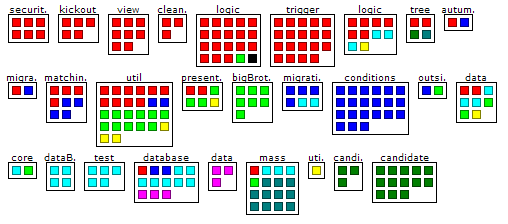
\includegraphics[width=\linewidth]{fig/hapax-outsight-distribution}\\
  \caption{The Distribution Map of Outsight, a webbased job portal application \cite{Kuhn06a}.}\label{fig:outsight}
\end{figure}

Only one topic out of nine concepts is about the system's domain: job exchange. Topic \red includes the complete domain of the system: that is users, companies and CVs. Whereas all other topics are application specific components: topic \blue is a CV search engine, topic \darkgreen implements PDF generation, topic \green is text and file handling, topic \cyan and \magenta provide access to the database, and topic DarkCyan is a testing and debugging facility. Additionally the cross-cutting topic \yellow bundles high-level clones related to time and timestamps.

\textbf{On the congruence between topics and packages.} In section \autoref{sec:distribution} we discussed the relation between topics and packages. Considering again the case study in \autoref{fig:outsight} as an example, we find occurrences of all four patterns: Topic \darkgreen for example is well-encapsulated, whereas topic \yellow cross-cuts the application. Then there is topic \blue, which is an octopus with the \emph{conditions} package as its body and tentacles reaching into six other packages, and finally we have in the \emph{logic} package an instance of a black sheep.

\textbf{On source documents that are related to more than one topic.} If we want to analyze how the topics are spread across some type of documents (\eg packages, classes or methods) we have to break the system into documents one level below the target level. For example, if we want to analyze the topic distribution over packages, we break the system into classes and analyze how the topics of classes are spread over the packages.

%%%%%%%%%%%%%%%%%%%%%%%%%%%%%%%%%%%%%%%%%%
\section{Conclusions}\label{sec:conclusions}
%%%%%%%%%%%%%%%%%%%%%%%%%%%%%%%%%%%%%%%%%%

Source code bears the semantics of an application in the names of identifiers and comments. In this chapter we present our approach to retrieve the topics present in the source code vocabulary to support program comprehension. We introduce lexical clustering, a technique based on Latent Semantic Indexing and clustering to group source documents that use similar vocabulary. We call these groups lexical clusters and we interpret them as linguistic topics that reveal the intention of the code. As compared to our previous approach, we go a step forward and use Distribution Maps to illustrate how the lexical clusters are distributed over the system.

We applied the approach on several case studies with different characteristics, two of which are presented in this chapter.  The case studies give evidence that our approach provides a useful first impression of an unfamiliar system, and that we reveal valuable developer knowledge. The Distribution Map together with the labeling provides a good first impression of the software's domain. Lexical clustering captures topics regardless of class hierarchies, packages and other structures. One can, at a glance, see whether the software covers just a few or many different topics, how these are distributed over the structure, and -- due to the labeling -- what they are about.

When starting this work, one of our hypotheses was that lexical clustering would reveal a systems domain semantics. However, our experiments showed that most linguistic topics relate to application concepts or architectural components. Usually, our approach partitions a system into one (or sometimes two) large domain-specific clusters and up to a dozen domain-independent clusters. As part of our future work, we plan to investigate more closely the relationship between linguistic topics and both domain and application concepts.

In the future we would also like to investigate in more depth recall and precision of the approach. For example, we would like to compare the results of the lexical clustering with other types of clustering. Furthermore, we would like to improve the labeling with other computer linguistic techniques.

%%%%%%%%%%%%%
%%%%%%%%%%%%%
%%%%%%%%%%%%%
%%%%%%%%%%%%%
%%%%%%%%%%%%%
%%%%%%%%%%%%%
%%%%%%%%%%%%%
%%%%%%%%%%%%%

\chapter{Code Summarization}
\label{the chapter on LogLR}

\infobox
	{Refinding and discovering topics}
	{Part of a system's codebase or history}
	{Lexcial and episodic (established through lexical information)}
	{Visual analytics of word clouds}

Source code rarely comes with an executive summary. When developers encounter a piece of source code for the first time, they are typically not presented with a high-level summary of the code's topics. Looking at package and class names might help to make an educated guess, but does often not give away the complete picture. Even the more, when comparing two pieces of source code or two entire systems to two versions of the same system, developers are missing a high-level summary that distilles the difference in a short textual summarization. The need for software summarization is obvious.

In the following chapter we present an approach to summarize part of a system as a word cloud, that consist of the statistically most significant terms that set this part of system apart from the rest. The same approach can be use to compare two parts of a system to compare two versions of the same system. When comparing version, both statistically significant addition and removals are shown using two different colors. Presenting those word clouds to the developer helps them to lexically query the topics, as well as when presenting all words clouds of a systems versions to recover and tell the story of a systems history and thus enabling developers to draw from episodic memories that they possibly never experiences first-hand themselves.

\asteriskasteriskasterisk

\todo{Include MSR Poster}

As more and more open-source software components become available on the internet we need automatic ways to label and compare them. For example, a developer who searches for reusable software must be able to quickly gain an understanding of retrieved components. This understanding cannot be gained at the level of source code due to the semantic gap between source code and the domain model. In this chapter we present a lexical approach that uses the log-likelihood ratios of word frequencies to automatically provide labels for software components. We present a prototype implementation of our labeling/comparison algorithm and provide examples of its application. In particular, we apply the approach to detect trends in the evolution of a software system.

In recent years, software vocabulary has been proven to be a valuable source for software analysis, often including the retrieval of labels (\eg \cite{Baldi08OOPSLA,EinarHoest,Kuhn07a}). However, labeling software is not without pitfalls. The distribution of words in software corpora follows the same power-law as word frequencies in natural-language text \cite{Linstead09SUITE}. Most of the text is made up of a small set of common terms, whereas content-bearing words are rare. Analysis of software vocabulary must deal with the reality of rare terms, thus statistical tests that assume normal distribution are not applicable. For example, textual comparison based on directly counting term frequencies is subject to overestimation when the frequencies involved are very small.  

For text analysis the use of \loglr improves the statistical results. Likelihood tests do not depend on assumptions of normal distribution, instead they use the asymptotic distribution of binomial likelihood \cite{Dunning}. Using \loglr{}s allows comparisons to be made between the significance of occurrences of both common and rare terms.

In this chapter we present a lexical approach that uses the \loglr of word frequencies to automatically retrieve labels from source code. The approach can be applied i) to compare components with each other, ii) to compare a component against a normative corpus, and iii) to compare different revisions of the same component. We present a prototype implementation and give examples of its application. In particular, we apply the approach to detect trends in the evolution of the JUnit software system.

\section{Log-Likelihood in a Nutshell}\label{nutshell}

This section explains how log-likelihood ratio is applied to analyse word frequencies. The explanations are kept as concise as possible. We provide the general background and just enough details such that a programmer may implement the algorithm. Please refer to Ted Dunning's work \cite{Dunning} for more background.

The idea behind \loglr is to compare two statistical hypotheses, of which one is a subspace of the other. Given two text corpora, we compare the hypothesis that both corpora have the same distribution of term frequencies with the ``hypothesis'' given by the actual term frequencies. Because we know that terms are not equally distributed over source code, we use binomial likelihood

$$ L(p,k,n) = p^k ( 1 - p) ^ { n - k }$$
\noindent
with $p = \frac{k}{n}$, where $k$ is the term frequency (\ie number of occurrences) and $n$ the size of the corpus. Taking the logarithm of the likelihood ratio gives
\footnote{In some publications (\eg \cite{Rayson}) we found that the last two terms were omitted (since their values tend to be orders of magnitude smaller than the corresponding values of the first two terms). The results presented in this chapter, however, are obtained using the complete log likelihood ratio formula.}

\begin{align*}
-2 \log \lambda =~&2 \big[ \log L(p_1,k_1,n_1) + \log L(p_2,k_2,n_2)\\
 &- \log L(p,k_1,n_1) - \log L(p,k_2,n_2) \big] 
\end{align*}
\noindent
with $p = \frac{k_1 + k_2}{n_1 + n_2}$. The higher the value of $-2log\lambda$ the more significant is the difference between the term frequencies in of both text corpora. By multiplying the $-2log\lambda$ value with the signum of $p_1 - p_2$ we can further distinguish between terms specific to the first corpus and terms specific to the second corpus. Terms that are equally frequent in both corpora have a $-2log\lambda$ value close to zero and thus fall in between.

\paragraph{Example.} Let $C_1$ be the corpus of a software project with size $n_1 = 10^6$, where the words \verb$`rare'$, \verb$`medium'$, and \verb$`common'$ appear respectively 1, 100, and $1\times10^4$ times; and let $C_2$ be the corpus of one of the project's classes with size $n_2 = 1000$, where each word appears 10 times. Then the \loglr{} values are

\begin{center}
\begin{tabular}{l | rrrr}
~ & $p_1$ & $p_2$ & $-2log\lambda$ & $\chi^2$ \\ 
\hline
\verb$rare$ & $10^{-6}$ & $10^{-2}$  & 131.58 & 9.08 \\
\verb$medium$ & $10^{-4}$ & $10^{-2}$  & 71.45 & 0.89 \\
\verb$common$ & $10^{-2}$ & $10^{-2}$  & 0.00 & 0.00 \\
\end{tabular}
\end{center}

The column $\chi^2$ lists the value of Pearson's chi-square test, which assumes normal distribution. As we can see, there is an overestimation when the frequencies involved are very small. Therefore, text analysis should use \loglr{}s to compare the occurrences of common and rare terms \cite{Dunning}.


\section{Applications}\label{applications}

In this section we present two example applications of log-likelihood ratio for software analysis.
There are two main types of corpus comparison: comparison of a sample corpus to a larger corpus, and comparison of a two equally sized corpora. In the first case, we refer to the large corpus as a \emph{normative} corpus since it provides as norm against which we compare.

Applications of these comparisons are
\begin{itemize}
\item \emph{Providing labels for components.} Comparing a component's vocabulary with a large normative corpus (as \eg Sourceforge, Github, or Sourcerer \cite{Bajrach09SUITE}), we obtain labels that describe the component. In the same way, we can compare a class's vocabulary against the containing project.
\item \emph{Comparing components to each other.} Comparing two components, we obtain labels to describe their differences as well as commonalities. This is applicable at any level of granularity, from the level of projects down to the level of methods.
\item \emph{Documenting the history of a component.} Comparing subsequent revisions of the same component, we obtain labels to describe the evolution of that component. (Using multinominal distribution we could even compare all revisions at once, although such results are harder to interpret \cite{Dunning}.)
\item \emph{Describing the results of software search.} Code-search engines have recently received much attention, both commercial engines (as \eg Krugle) and academic engines (as \eg Sourcerer \cite{Bajrach09SUITE}) are publicly available. The result of a search query are typically provided by presenting a peep-hole view on the matching source line and its context to the user. Comparing each result, or the class/project that contains the result, against the entire index we can provide labels that may help users to make better use of these results.
\item \emph{Analysing the structural use of vocabulary.} There has been much confusion regarding which parts of the software vocabulary are to be considered in software analysis. Some approaches consider the entire source code including comments, keywords and literals (\eg \cite{Kuhn08b,Kuhn07a}), other approaches consider class and methods names only (\eg \cite{Baldi08OOPSLA,EinarHoest}). A recent study compared the vocabulary of different structural level using techniques that assume normal distribution \cite{Linstead09SUITE}. Log-likelihood ratios provide a statistically more sound means to study these phenomena.
\end{itemize}

\noindent We implemented $-2log\lambda$ analysis in a Java prototype which is available on the \textsc{Hapax} website\footnote{\url{http://smallwiki.unibe.ch/adriankuhn/hapax}} under AGPL license. In the remainder of this section we present results obtained with that prototype.

\subsection{Labeling the Java API}\label{example1}

\begin{table}
{\scriptsize \begin{center}
\begin{tabular}{lr | lr | lr}
\verb$java.io$ & ~ & \verb$java.text$ & ~ &  \verb$java.util$ & ~ \\
\hline
read & 521.99 & pattern & 228.92 & iterator & 306.91\\
write & 481.93 & format & 209.40 & entry & 301.90\\
skip & 154.61 & digits & 183.24 & next & 237.82\\
close & 113.41 & FIELD & 167.58 & E & 222.33\\
mark & 111.47 & instance & 127.16 & contains & 187.69\\
println & 99.66 & fraction & 104.98 & sub & 166.49\\
UTF & 85.27 & integer & 102.77 & of & 165.57\\
flush & 80.96 & index & 93.43 & K & 154.07\\
desc & 69.19 & run & 90.99 & T & 154.30\\
TC & 68.88 & currency & 91.55 & key & 145.10\\
prim & 61.48 & decimal & 86.34 & all & 145.74\\
char & 61.28 & contract & 84.92 & V & 142.15\\
buf & 60.15 & separator & 72.11 & remove & 128.59\\
stream & 56.86 & grouping & 62.26 & last & 128.09\\
fields & 52.38 & parse & 56.93 & map & 115.68\\
bytes & 47.99 & collation & 56.60 & clear & 114.03\\
\dots & ~ & \dots & ~ & \dots & ~ \\
border & -28.35 & UI & -23.07 & create & -62.67\\
set & -33.89 & border & -22.77 & listener & -62.42\\
remove & -37.49 & property & -24.23 & action & -63.83\\
listener & -39.79 & remove & -30.11 & UI & -64.68\\
accessible & -40.97 & accessible & -32.91 & border & -63.83\\
paint & -44.90 & listener & -31.97 & accessible & -92.25\\
value & -59.10 & type & -32.18 & paint & -101.11\\
get & -64.38 & paint & -36.07 & get & -164.14\\
\end{tabular}
\end{center}}
\caption{Labels retrieved for three Java packages using the full Java 6.0 API as normative corpus.}
\label{tab:one}
\end{table}%


In this example, we compare the packages \verb$java.io$ and \verb$java.text$ and \verb$java.util$ with the normative corpus of the full Java 6.0 API. We use the Java Compiler (JSR 199) to parse the byte-code of the full Java API and then extract the vocabulary of all public and protected elements. We extract the names of packages, classes (including interfaces, annotations, and enums), fields, methods and type parameters. We split the extracted names by camel-case to accomodate to the Java naming convention.

Results are shown in \autoref{tab:one}. For each package we list the most specific words and the least specific words. All three packages are characterized by not covering UI code, in addition \verb$java.io$ and \verb$java.util$ have obviously substantially fewer \verb$get$-accessors than is usual for the Java API. The remaining findings offer no further surprises, except maybe for the uppercase letters in \verb$java.util$ which are generic type parameters; obviously the majority of the Java 6.0 API makes less use of generic types than the collection framework.

%\subsection{Compare Components to Each Other}\label{example2}

%In this example, we compare the \verb$JUnit$ project to the \verb$JExample$ project, both of which are unit testing frameworks. We parse the source code of both projects and extract the complete vocabulary, including comments and literals. We split the extracted words by camel-case to accomodate to the Java naming convention, and apply stemming. We do not, however, exclude common keywords (as \eg \verb$public$ and \verb$float$) since learning about the different use of keywords is a valuable insight as well. 

\subsection{The Evolution of JUnit}\label{example3}

In this example, we report on the vocabulary trends in the history of the \verb$JUnit$\footnote{\url{http://www.junit.org}} project. We use a collection of 14 release distributions of JUnit and parse the source code of each release.  We compare the vocabulary of each two subsequent releases and report on the most significant changes in the vocabulary. We extract all words, including comments; split by camel-case, and exclude English stopwords but not Java keywords.

Results are shown in \autoref{tab:two}. For each release we list the top removed terms and the top added terms, as well as the $-2log\lambda$ value of the top-most term. Large $-2log\lambda$ values indicate substantial changes.

The top 7 change trends (\ie $-2log\lambda \geqslant 100.0$) in the history of JUnit are as follows. In 3.2 removal of \verb$MoneyBag$ example and introduction of graphical UI; in 4.0 removal of graphical UI and introduction of annotation processing; in 4.2 removal of HTML tags from Javadoc comments; in 4.4 introduction of theory matchers and \verb$hamcrest$ framework; in 4.5 introduction of blocks and statements. We manually verified these findings with the release notes of JUnit and found that the findings are appropriate.
 
\begin{table}
{\scriptsize \begin{center}
\begin{tabular}{lrl}
\textbf{JUnit} & $2log\lambda$ & \textbf{Top-10 terms (with $-2log\lambda \geqslant10.0$)} \\
\hline
3 & -8.21 &  \\
~ & 54.11 & count, writer, wrapper \\
\hline
3.2 & -382.80 & money, CHF, assert, case, USD, equals, test, fmb,\\~&~& result, currency \\
~ & 114.21 & tree, model, constraints, combo, reload, swing,\\~&~& icon, pane, browser, text \\
\hline
3.4 & -19.48 & stack, util, button, mouse \\
~ & 15.73 & preferences, base, zip, data, awtui \\
\hline
3.5 & -38.78 & param, reload, constraints \\
~ & 69.34 & view, collector, context, left, cancel, values,\\~&~& selector, views, icons, display \\
\hline
3.6 & -1.20 &  \\
~ & 8.72 &  \\
\hline
3.7 & -8.25 &  \\
~ & 2.79 &  \\
\hline
3.8 & -13.30 & deprecated \\
~ & 23.40 & printer, boo, lines \\
\hline
4.0 & -349.34 & constraints, grid, bag, set, label, panel, path,\\~&~& icon, model, button \\
~ & 350.47 & description, code, nbsp, org, annotation,\\~&~& notifier, method, request, runner, br \\
\hline
4.1 & -1.43 &  \\
~ & 61.90 & link, param, check \\
\hline
4.2 & -288.53 & nbsp, br \\
~ & 20.03 & link, builder, pre, li \\
\hline
4.3.1 & -8.91 &  \\
~ & 53.36 & array, actuals, expecteds, multi, dimensional,\\~&~& arrays, values, javadoc \\
\hline
4.4 & -34.32 & introspector, code, todo, multi, javadoc,\\~&~& dimensional, array, runner, test, fix \\
~ & 151.98 & matcher, theories, experimental, hamcrest,\\~&~& matchers, theory, potential, item, supplier,\\~&~& parameter \\
\hline
4.5 & -30.11 & theory, theories, date, result, static, validator,\\~&~& pointer, string, assert, experimental \\
~ & 124.28 & statement, model, builder, assignment, block,\\~&~& errors, unassigned, evaluate, describable,\\~&~& statements \\
\end{tabular}
\end{center}}
\caption{Evolution of JUnit: for each release we list the removed and the added words, large $2log\lambda$ values indicate more significant changes.}
\label{tab:two}
\end{table}%

%\subsection{On the Structural Use of Vocabulary}\label{example5}

%In this example, we take again the Java API of version 1.6 as case study. We group the extracted names by structural category: package names, class names (which are further subdivided in class and interface names), method names, and field names. As in the first example, we use the Java Compiler API (JSR 199) to parse the binaries and extract the vocabulary of all public and protected elements. We proceed with split by camel-case and stemming.

%\todo{Fill in epic table with results.}

%\todo{Compare the results to Linstead's work.}

\section{Conclusion}\label{eventually}

We presented \loglr as a technique to label software components. Using \loglr{}s allows comparisons to be made between the significance of occurrences of both common and rare terms. We presented how to use the \loglr of word frequencies to retrieve labels, and how to compare a component against a normative corpus. In addition, we proposed to use \loglrs to characterize the evolution of a software component. We presented the results of two example applications, one using the Java API as case study, the other using 14 releases of JUnit as case study. By comparing subsequent revisions of JUnit to each other we were able to characterize substantial changes in the history of JUnit.

%%%%%%%%%%%%%
%%%%%%%%%%%%%
%%%%%%%%%%%%%
%%%%%%%%%%%%%
%%%%%%%%%%%%%
%%%%%%%%%%%%%
%%%%%%%%%%%%%
%%%%%%%%%%%%%

\chapter{Stories of Collaboration}
\label{the chapter on chronia}

\infobox
	{Learning about team collaboration}
	{Team of a project's local codebase}
	{Episodic (established through social and historical information)}
	{Visual analytics of a story-telling visualization}

Episodic cues are of great help to developers when having to find their way through a system, whoever episodic memory is only available to those developer that know the system's history first-hand. For most software systems, the tribal folklore of the team is the only record on the system's history beside the version control system. The tribal folklore is hard to query because it is only present as the team's episodic memory, and the version control system is hard to query because it is typically only present as a series of textual low-level changes to the systems source code. There is a need for better means of recovering and telling a systems story to both new hires and seasoned team members.

In the following chapter we present an approach to visualization a system history and its team's collaboration as a story-telling visualization. Story-telling visualizations are a branch of information visualization that has been popularized by the political information graphics of newspapers such as the New York Times and the Guardian. A story-telling visualization is supposed to invite its reader to get engaged with the visualized data by establishing a personal connection between the reader and the presented data. Our approach uses social and historical information taken from the version control system to establish an episodic visualization of the system's history. We show the lifeline of files ordered by code ownership, thus telling the story of the team's collaboration. Team are typically getting very engaged and excited when showen the visualization of their own system. Both new hires and seasoned team members can use this visualization to learn about episodes from the system's history in order to take better technical decisions when working with the system in the future.

\asteriskasteriskasterisk

As systems evolve their structure change in ways not expected upfront. As time goes by, the knowledge of the developers becomes more and more critical for the process of understanding the system. That is, when we want to understand a certain issue of the system we ask the knowledgeable developers. Yet, in large systems, not every developer is knowledgeable in all the details of the system. Thus, we would want to know which developer is knowledgeable in the issue at hand. In this chapter we make use of the mapping between the changes and the author identifiers (\eg user names) provided by versioning repositories. We first define a measurement for the notion of code ownership. We use this measurement to define the \omap visualization to understand when and how different developers interacted in which way and in which part of the system\footnote{The visualizations in this chapter make heavy use of colors. Please obtain a color-printed or electronic version for better understanding.}. We report the results we obtained on several large systems.

Software systems need to change in ways that challenge the original design. Even if the original documentation exists, it might not reflect the code anymore. In such situations, it is crucial to get access to developer knowledge to understand the system. As systems grow larger, not all developers know about the entire system, thus, to make the best use of developer knowledge, we need to know which developer is knowledgeable in which part of the system.

From another perspective, Conway's law \cite{Conw68a} states that ``Organizations which design systems are constrained to produce designs which are copies of the communication structures of these organizations." That is, the shape of the organization reflects on the shape of the system. As such, to understand the system, one also has to understand the interaction between the developers and the system \cite{Deme02a}.

In this chapter we aim to understand how the developers drove the evolution of the system. In particular we provide answers to the following questions:
\begin{itemize}
\item How many authors developed the system?
\item Which author developed which part of the system?
\item What were the behaviors of the developers?
\end{itemize}

In our approach, we assume that the original developer of a line of code is the most knowledgeable in that line of code. We use this assumption to determine the owner of a piece of code (\eg a file) as being the developer that owns the largest part of that piece of code. We make use of the ownership to provide a visualization that helps to understand how developers interacted with the system. The visualization represents files as lines, and colors these lines according to the ownership over time.

Contrary to similar approaches \cite{Ryss04a}, we give a semantic order to the file axis (\ie we do not rely on the names of the files) by clustering the files based on their history of changes: files committed in the same period are related \cite{Gall98a}.

We implemented our approach in Chronia, a tool built on top of the Moose reengineering environment \cite{Duca05a}. As CVS is a de facto versioning system, our implementation relies on the CVS model. Our aim was to provide a solution that gives fast results, therefore, our approach relies only on information from the CVS log without checking out the whole repository. As a consequence, we can analyze large systems in a very short period of time, making the approach usable in the early stages of reverse engineering.

To show the usefulness of our solution we applied it on several large case studies. We report here some of the findings and discuss different facets of the approach.

The contributions of the chapter are:
\begin{itemize}
\item The definition of file ownership.
\item The clustering of files based on their commit history.
\item A characterization of developer behaviors.
\item The \omap visualization.
\end{itemize}

%%%%%%%%%%%%%%%%%%%%%%%%%%%%%%%%%%%%%%%%%%%%%%%%%%%
\section{Data Extraction from CVS log}\label{sec:ownership}
%%%%%%%%%%%%%%%%%%%%%%%%%%%%%%%%%%%%%%%%%%%%%%%%%%%

This section introduces a measurement to characterize the code ownership. The assumption is that the original developer of a line of code is the most knowledgeable in that line of code. Based on this assumption, we determine the owner of a piece of code as being the developer that owns the most lines  of that piece of code.

The straightforward approach is to checkout all file versions ever committed to the versioning repository and to compute the code ownership from diff information between each subsequent revisions $f_{n-1}$ and $f_n$. From an implementation point of view this implies the transfer of large amounts of data over the network, and long computations.

In this chapter, we aim to provide for an approach that can deal with large projects with long history, and that can provide the results fast. As CVS is the very common versioning system, we make tuned our approach to work with the information CVS can provide. In particular we compute the ownership of the code based only on the CVS log information.

Below we present a snippet from a CVS log. The log lists for each version $f_n$ of a file \-- termed revision in CVS \-- the time $t_{f_n}$ of its commit, the name of its author $\alpha_{f_n}$, some state information and finally the number of added and removed lines as deltas $a_{f_n}$ and $r_{f_n}$. We use these numbers to recover both the file size $s_{f_n}$, and the code ownership $own_{f_n}^\alpha$.

\begin{tiny}\begin{verbatim}
----------------------------
revision 1.38
date: 2005/04/20 13:11:24;  author: girba;  state: Exp;  lines: +36 -11
added implementation section
----------------------------
revision 1.37
date: 2005/04/20 11:45:22;  author: akuhn;  state: Exp;  lines: +4 -5
fixed errors in ownership formula
----------------------------
revision 1.36
date: 2005/04/20 07:49:58;  author: mseeberg;  state: Exp;  lines: +16 -16
Fixed math to get pdflatex through without errors.
----------------------------
\end{verbatim}\end{tiny}

%%%%%%%%%%%%%%%%%%%%%%%%%%%%%%%%%%%%%%%%%%%%%%%%%%%
\subsection{Measuring File Size}
%%%%%%%%%%%%%%%%%%%%%%%%%%%%%%%%%%%%%%%%%%%%%%%%%%%

Let $s_{f_n}$ be the size of revision $f_n$, measured in number of lines. The number of lines is not given in the CVS log, but can be computed from the deltas $a_{f_n}$ and $r_{f_n}$ of added and removed lines. Even though the CVS log does not give the initial size $s_{f_0}$, we can give an estimate based on the fact that one cannot remove more lines from a file than were ever contained. We define $s_{f_n}$ as in autoref{fig:filesize}: we first calculate the sizes starting with an initial size of 0, and then in a second pass adjust the values with the lowest value encountered in the first pass.

\begin{figure}[htbp]
\begin{minipage}[c]{.45\linewidth}
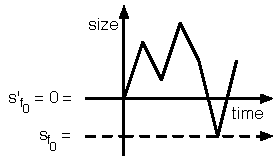
\includegraphics[width=1.2\linewidth]{fig/chronia-minimum}
 \end{minipage}
 \hfill
 \begin{minipage}[c]{.5\linewidth}
\begin{eqnarray}
& s'_{f_0} := 0 \nonumber \\
& s'_{f_n} := s'_{f_{n-1}} + a_{f_{n-1}} - r_{f_n} \nonumber  \\
& s_{f_0} := \vert min \{ s'_x \} \vert \nonumber \\
& s_{f_n} := s_{f_{n-1}} + a_{f_n} - r_{f_n} \nonumber
 \end{eqnarray}
 \end{minipage}
\caption{The computation of the initial size.}
\label{fig:filesize}
\end{figure}

This is a pessimistic estimate, since lines that never changed are not covered by the deltas in the CVS log. This is an acceptable assumption since our main focus is telling the story of the developers, not measuring lines that were never touched by a developer. Furthermore in a long-living system the content of files is entirely replaced or rewritten at least once if not several times. Thus the estimate matches the correct size of most files.

%%%%%%%%%%%%%%%%%%%%%%%%%%%%%%%%%%%%%%%%%%%%%%%%%%%
\subsection{Measuring Code Ownership}
%%%%%%%%%%%%%%%%%%%%%%%%%%%%%%%%%%%%%%%%%%%%%%%%%%%

A developer owns a line of code if he was the last one that committed a change to that line. In the same way, we define file ownership as the percentage of lines he owns in a file. And the overall owner of a file is the developer that owns the largest part of it.

Let $own_{f_n}^\alpha$ be the percentage of lines in revision $f_n$ owned by author $\alpha$. Given the file size $s_{f_n}$, and both the author $\alpha_{f_n}$ that committed the change and $a_{f_n}$ the number of lines he added, we defined ownership as:
\[
own_{f_0}^\alpha:=\left\{
    \begin{array}{cl}
        1, & \alpha=\alpha_{f_0} \\
        0, & else
    \end{array}\right.
\]
\[
own_{f_n}^\alpha:=own_{f_{n-1}}^\alpha \frac{s_{f_n} - a_{f_n}}{s_{f_n}} + \left\{
    \begin{array}{cl}
        \frac{a_{f_n}}{s_{f_n}}, & \alpha=\alpha_{f_n} \\
        0, & else
    \end{array}\right.
\]
In the definition we assume that the removed lines $r_{f_n}$ are evenly distributed over the ownership of the preceding owners of $f_{n-1}$.
%A better estimate than $own_{f_n}^\alpha$ can be retrieved by checking out the content of each revision and using a diff algorithm to find out to whom the removed lines actually belonged. But this would, as initially explained, require vast amounts of network traffic and time consuming calculations, and thus the advantages of only processing information from CVS log would be lost.

%%%%%%%%%%%%%%%%%%%%%%%%%%%%%%%%%%%%%%%%%%%%%%%%%%%
\section{The Ownership Map View}\label{sec:approach}
%%%%%%%%%%%%%%%%%%%%%%%%%%%%%%%%%%%%%%%%%%%%%%%%%%%

We introduce the \omap visualization as in autoref{fig:ownershipDetailsExample}. The visualization is similar to the Evolution Matrix \cite{Lanz02a}: each line represents a history of a file, and each circle on a line represents a change to that file.

The color of the circle denotes the author that made the change. The size of the circle reflects the proportion of the file that got changed \ie the larger the change, the larger the circle. And the color of the line denotes the author who owns most of the file.

Bertin \cite{Bert74a} assessed that one of the good practices in information visualization is to offer to the viewer visualizations that can be grasped at one glance. The colors used in our visualizations follow visual guidelines suggested by Bertin, Tufte \cite{Tuft90a}, and Ware \cite{Ware00a} \-- \eg we take into account that the human brain is not capable of processing more than a dozen distinct colors.

In a large system, we can have hundreds of developers. Because the human eye is not capable of distinguishing that many colors, we only display the authors who committed most of all changes using distinct colors; the remaining authors are represented in gray. Furthermore, we also represent with gray files that came into the CVS repository with the initial import, because these files are usually sources from another project with unknown authors and are thus not necessarily created by the author that performed the import. In short, a gray line represents either an unknown owner, or an unimportant one.

\begin{figure}[htb]
\begin{center}
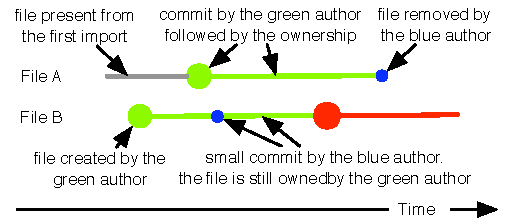
\includegraphics[width=\linewidth]{fig/hapax-owners-map-detail.pdf}
\caption{Example of ownership visualization of two files.}
\label{fig:ownershipDetailsExample}
\end{center}
\end{figure}

In the example from autoref{fig:ownershipDetailsExample}, each line represents the lifetime of a file; each circle represents a change. \id{File A} appears gray in the first part as it originates from the initial import. Later the green author significantly changed the file, and he became the owner of the file. In the end, the blue author deleted the file. \id{File B} was created by the green author. Afterwards, the blue author changed the file, but still the green author owns the larger part, so the line remains green. At some point, the red author committed a large change and took over the ownership. The file was not deleted.

\begin{figure*}[hbt]
\begin{center}
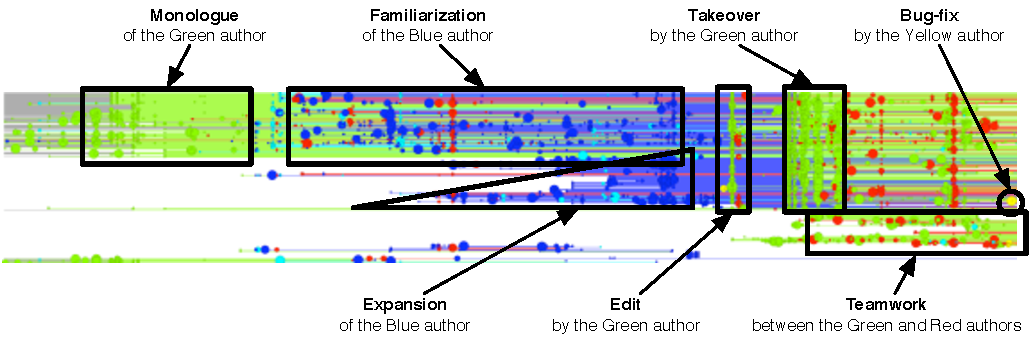
\includegraphics[width=\linewidth]{fig/hapax-owners-map-example}
\caption{Example of the Ownership Map view. The view reveals different patterns:
Monologue, Familiarization, Edit, Takeover, Teamwork, Bug-fix.}
\label{fig:ownershipMapExample}
\end{center}
\end{figure*}

%%%%%%%%%%%%%%%%%%%%%%%%%%%%%%%%%%%%%%%%%%%%%%%%%%%
\subsection{Ordering the Axes}
%%%%%%%%%%%%%%%%%%%%%%%%%%%%%%%%%%%%%%%%%%%%%%%%%%%

\paragraph{Ordering the Time Axis.}
Subsequent file revisions committed by the same author are grouped together to form a transaction of changes \ie a commit. We use a single linkage clustering with a threshold of 180 seconds to obtain these groups. This solution is similar to the sliding time window approach of Zimmerman \etal when they analyzed co-changes in the system \cite{Zimm04a}. The difference is that in our approach the revisions in a commit do not have to have the same log comment, thus any quick subsequent revisions by the same author are grouped into one commit.

\paragraph{Ordering the Files Axis.}
A system may contain thousands of files; furthermore, an author might change multiple files that are not near each other if we would represent the files in an alphabetical order. Likewise, it is important to keep an overview of the big parts of the system. Thus, we need an order that groups files with co-occurring changes near each other, while still preserving the overall structure of the system. To meet this requirement we split the system into high-level modules (\eg the top level folders), and order inside each module the files by the similarity of their history. To order the files in a meaningful way, we define a distance metric between the commit signature of files and order the files based on a hierarchical clustering.

Let $H_f$ be the commit signature of a file, a set with all timestamps $t_{f_n}$ of each of its revisions $f_n$. Based on this the distance between two commit signatures $H_a$ and $H_b$ can be defined as the modified Hausdorff distance \footnote{The Hausdorff metric is named after the german mathematician Felix Hausdorff (1868-1942) and is used to measure the distance between two sets with elements from a metric space.} $\delta(H_a,H_b)$:
\[
D(H_n,H_m) := \sum_{n \in H_n} min^2 \{ \vert m -n \vert : m \in H_m \}
\]
\[
\delta(H_a,H_b) := max \{ D(H_a,H_b), D(H_b,H_a) \}
\]

With this metric we can order the files according to the result of a hierarchical clustering algorithm \cite{Jain99a}. From this algorithm a dendrogram can be built: this is a hierarchical tree with clusters as its nodes and the files as its leaves. Traversing this tree and collecting its leaves yields an ordering that places files with similar histories near each other and files with dissimilar histories far apart of each other.

The files axes of the \omap views shown in this chapter are ordered with \textit{average linkage} clustering and \textit{larger-clusters-first} tree traversal. Nevertheless, our tool Chronia allows customization of the ordering.

%%%%%%%%%%%%%%%%%%%%%%%%%%%%%%%%%%%%%%%%%%%%%%%%%%%
\subsection{Behavioral Patterns}
%%%%%%%%%%%%%%%%%%%%%%%%%%%%%%%%%%%%%%%%%%%%%%%%%%%

The Overview Map reveals semantical information about the work of the developer. autoref{fig:ownershipMapExample} shows a part of the \omap of the Outsight case study (for more details see  autoref{sec:outsight}). In this view we can identify several different behavioral patterns of the developers:

\begin{itemize}

\item \emph{Monologue.} Monologue denotes a period where all changes and most files belong to the same author. It shows on an \omap as a unicolored rectangle with change circles in the same color.

\item \emph{Dialogue.} As opposed to Monologue, Dialogue denotes a period with changes done by multiple authors and mixed code ownership. On an \omap it is denoted by rectangles filled with circles and lines in different colors.

\item \emph{Teamwork.} Teamwork is a special case of Dialogue, where two or more developers commit a quick succession of changes to multiple files. On an \omap it shows as circles of alternating colors looking like a bunch of bubbles. In our example, we see in the bottom right part of the figure a collaboration between Red and Green.

\item \emph{Silence.} Silence denotes an uneventful period with nearly no changes at all. It is visible on an \omap as a rectangle with constant line colors and none or just few change circles.

\item \emph{Takeover.} Takeover denotes a behavior where a developer takes over a large amount of code in a short amount of time \-- \ie the developer seizes ownership of a subsystem in a few commits. It is visible on an \omap as a vertical stripe of single color circles together with an ensuing change of the lines to that color. A Takeover is commonly followed by subsequent changes done by the same author. If a Takeover marks a transition from activity to Silence we classify it as an \emph{Epilogue}.

\item \emph{Familiarization.} As opposed to Takeover, Familiarization characterizes an accommodation over a longer period of time. The developer applies selective and small changes to foreign code, resulting in a slow but steady acquisition of the subsystem. In our example, Blue started to work on code originally owned by Green, until he finally took over ownership.

\item \emph{Expansion.} Not only changes to existing files are important, but also the expansion of the system by adding new files. In our example, after Blue familiarized himself with the code, he began to extend the system with new files.

\item \emph{Cleaning.} Cleaning is the opposite of expansion as it denotes an author that removes a part of the system. We do not see this behavior in the example.

\item \emph{Bugfix.} By bug fix we denote a small, localized change that does not affect the ownership of the file. On an \omap it shows as a sole circle in a color differing from its surrounding.

\item \emph{Edit.} Not every change necessarily fulfills a functional role. For example, cleaning the comments, changing the names of identifiers to conform to a naming convention, or reshaping the code are sanity actions that are necessary but do not add functionality. We call such an action \emph{Edit}, as it is similar to the work of a book editor. An Edit is visible on an \omap as a vertical stripe of unicolored circles, but in difference to a Takeover neither the ownership is affected nor is it ensued by further changes by the same author. If an Edit marks a transition from activity to Silence we classify it as an \emph{Epilogue}.

\end{itemize}

%%%%%%%%%%%%%%%%%%%%%%%%%%%%%%%%%%%%%%%%%%%%%%%%%%%
\section{Validation}\label{sec:validation}
%%%%%%%%%%%%%%%%%%%%%%%%%%%%%%%%%%%%%%%%%%%%%%%%%%%

We applied our approach on several large case studies: Outsight, Ant, Tomcat, JEdit and JBoss. Due to the space limitations we report the details from the Outsight case study, and we give an overall impression on the other four well-known open-source projects.

\textbf{Outsight.} Outsight is a commercial web application written in Java and JSP. The CVS repository goes back three years and spans across two development iterations separated by half a year of maintenance. The system is written by four developers and has about 500 Java classes and about 500 JSP pages.

\textbf{Open-source Case Studies.} We choose Ant, Tomcat, JEdit, and JBoss to illustrate different fingerprints systems can have on an \omap. Ant has about 4500 files, Tomcat about 1250 files, JEdit about 500 files, and JBoss about 2000 files. The CVS repository of each project goes back several years.

%%%%%%%%%%%%%%%%%%%%%%%%%%%%%%%%%%%%%%%%%%%%%%%%%%%
\subsection{Outsight}\label{sec:outsight}
\begin{figure}[htbp]
\begin{center}
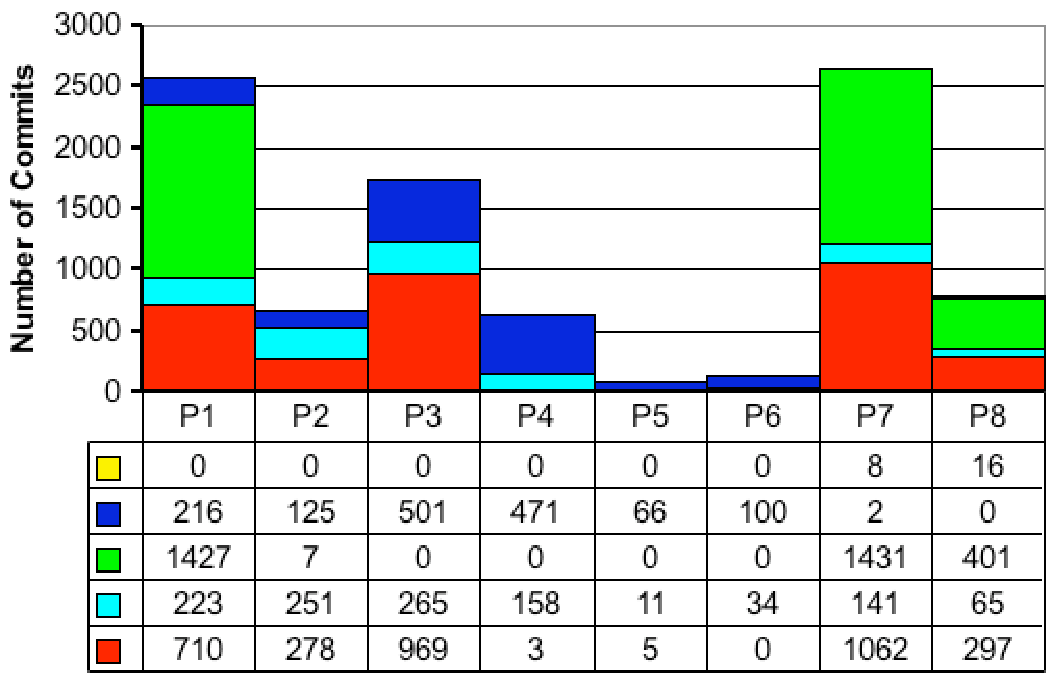
\includegraphics[width=\columnwidth]{fig/chronia-commit-histogram}
\caption{Number of commits per team member in periods of three months.}
\label{fig:histogram}
\end{center}
\end{figure}

\begin{figure*}[htbp]
\begin{center}
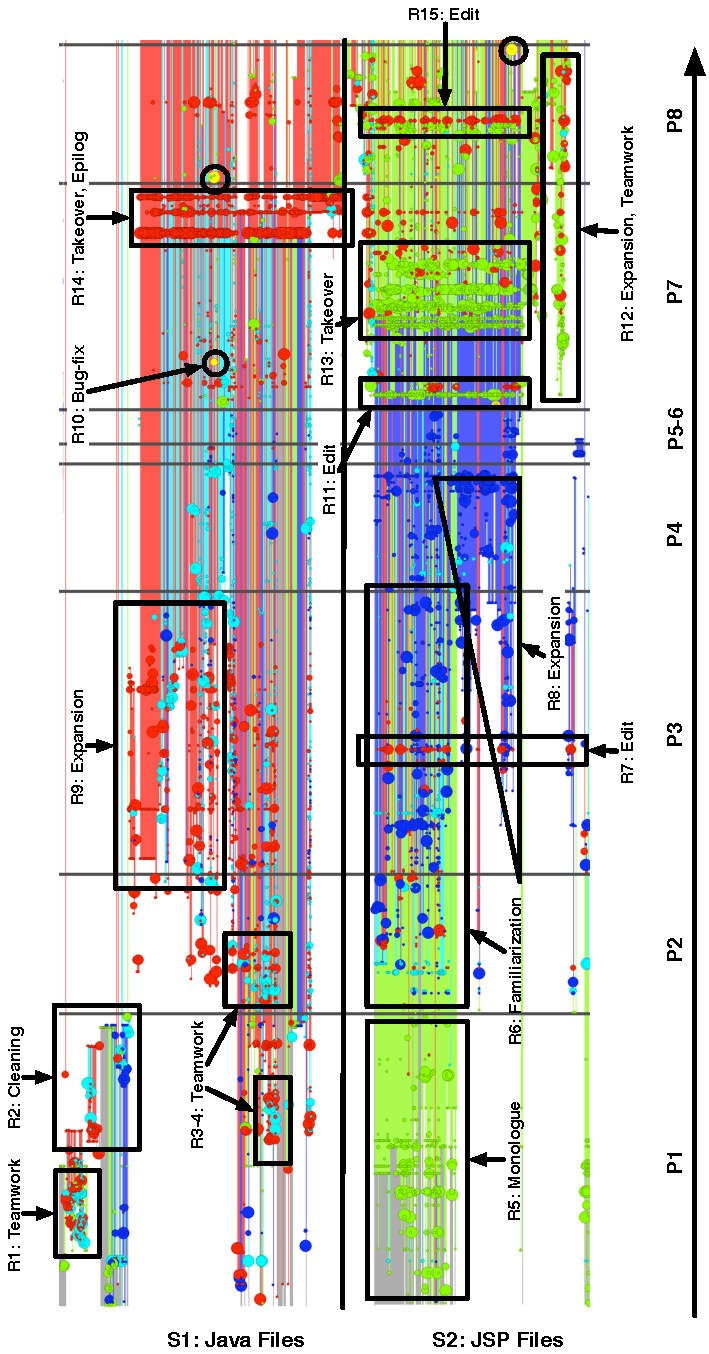
\includegraphics[height=21.3cm]{fig/chronia-outsight}
\caption{The Ownership Map of the Outsight case study.}
\label{fig:casestudy-outsight}
\end{center}
\end{figure*}

The first step to acquire an overview of a system is to build a histogram of the team to get an impression about the fluctuations of the team members over time. autoref{fig:histogram} shows that a team of four developers is working on the system. There is also a fifth author contributing changes in the last two periods only.



autoref{fig:casestudy-outsight} shows the \omap of our case study. The upper half are Java files, the bottom half are JSP pages. The files of both modules are ordered according to the similarity of their commit signature. For the sake of readability we use \id{S1} as a shorthand for the Java files part of the system, and \id{S2} as a shorthand for the JSP files part. Time is cut into eight periods \id{P1} to \id{P8}, each covering three months. The paragraphs below discuss each period in detail, and show how to read the \omap in order to answer our initial questions.

The shorthands in parenthesis denote the labels \id{R1} to \id{R15} as given on autoref{fig:casestudy-outsight}.

\textbf{Period 1.} In this period four developers are working on the system. Their collaboration maps the separation of \id{S1} and \id{S2}: while Green is working by himself on \id{S2} (\id{R5}), the others are collaborating on \id{S1}. This is a good example of Monologue versus Dialogue. A closer look on \id{S1} reveals two hotspots of Teamwork between Red and Cyan (\id{R1,R3}), as well as large mutations of the file structure. In the top part multiple Cleanings happen (\id{R2}), often accompanied by Expansions in the lower part.

\textbf{Period 2.} Green leaves the team and Blue takes over responsibility of \id{S2}. He starts doing this during a slow Familiarization period (\id{R6}), which lasts until end of \id{P3}. In the meantime Red and Cyan continue their Teamwork on \id{S1} (\id{R4}) and Red starts adding some files, which foreshadow the future Expansion in \id{P3}.

\textbf{Period 3.} This period is dominated by a big growth of the system, the number of files doubles as large Expansions happen in both \id{S1} and \id{S2}. The histogram in autoref{fig:histogram} identifies Red as the main contributor. The Expansion of \id{S1} evolves in sudden steps (\id{R9}), and as their file base grows the Teamwork between Red and Cyan becomes less tight. In contradiction the Expansion of \id{S2} evolves in small steps (\id{R8}), as Blue continues familiarizing himself with \id{S2} and slowly but steady takes over ownership of most files in this subsystem (\id{R6}). Also an Edit of Red in \id{S2} can be identified (\id{R7}).

\textbf{Period 4.} Activity moves down from \id{S1} to \id{S2}, leaving \id{S1} in a Silence only broken by selective changes. autoref{fig:histogram} shows that Red left the team, which consists now of Cyan and Green only. Cyan acts as an allrounder providing changes to both \id{S1} and \id{S2}, and Blue is further working on \id{S2}. The work of Blue culminates in an Epilogue marking the end of this period (\id{R8}). He has now completely taken over ownership of \id{S2}, while the ownership of subsystem \id{S1} is shared between Red and Cyan.

\textbf{Period 5 and 6.} Starting with this period the system goes into maintenance. Only small changes occur, mainly by author Blue.

\textbf{Period 7.} After two periods of maintenance the team resumes work on the system. In autoref{fig:histogram} we see how the composition of the team changed: Blue leaves and Green comes back. Green restarts with an Edit in \id{S2} (\id{R11}), later followed by a quick sequence of Takeovers (\id{R13}) and thus claiming back the ownership over his former code. Simultaneous he starts expanding \id{S2} in Teamwork with Red (\id{R12}).

First we find in \id{S1} selective changes by Red and Cyan scattered over the subsystem, followed by a period of Silence, and culminating in a Takeover by Red in the end \ie an Epilogue (\id{R14}). The Takeover in \id{S1} stretches down into \id{S2}, but there being a mere Edit. Furthermore we can identify two selective Bug-fixes (\id{R10}) by author Yellow, being also a new team member.

\textbf{Period 8.} In this period, the main contributors are Red and Green: Red works in both \id{S1} and \id{S2}, while green remains true to \id{S2}. As Red finished in the previous period his work in \id{S1} with an Epilogue, his activity now moves down to \id{S2}. There we find an Edit (\id{R15}) as well as the continuation of the Teamwork between Red and Green (\id{R12}) in the Expansion started in \id{P7}. Yet again, as in the previous period, we find small Bug-fixes applied by Yellow.

To summarize these finding we give a description of each author's behavior, and in what part of the system he is knowledgeable.

\textbf{Red author.} Red is working mostly on \id{S1}, and acquires in the end some knowledge of \id{S2}. He commits some edits and may thus be a team member being responsible for ensuring code quality standards. As he owns a good part of \id{S1} during the whole history and even closed that subsystem end of \id{P7} with an Epilogue, he is the developer most knowledgeable in \id{S1}.

\textbf{Cyan author.} Cyan is the only developer that was in the team during all periods, thus he is the developer most familiar with the history of the system. He worked mostly on \id{S1} and he owned large parts of this subsystem till end of \id{P7}. His knowledge of \id{S2} depends on the kind of changes Red introduced in his Epilogue. A quick look into the CVS log messages reveals that Red's Epilogue was in fact a larger than usual Edit and not a real Takeover: Cyan is as knowledgeable in \id{S1} as Red.

\textbf{Green author.} Green only worked in \id{S2}, and he has only little impact on \id{S1}. He founded \id{S2} with a Monologue, lost his ownership to Blue during \id{P2} to \id{P6}, but in \id{P7} he claimed back again the overall ownership of this subsystem. He is definitely the developer most knowledgeable with \id{S2}, being the main expert of this subsystem.

\textbf{Blue author.} Blue left the team after \id{P4}, thus he is not familiar with any changes applied since then. Furthermore, although he became an expert of \id{S2} through Familiarization, his knowledge might be of little value since Green claimed that subsystem back with multiple Takeovers and many following changes.

\textbf{Yellow author.} Yellow is a pure Bug-fix provider.

%%%%%%%%%%%%%%%%%%%%%%%%%%%%%%%%%%%%%%%%%%%%%%%%%%%
\subsection{Ant, Tomcat, JEdit and JBoss}

\begin{figure*}[htb]
\begin{center}
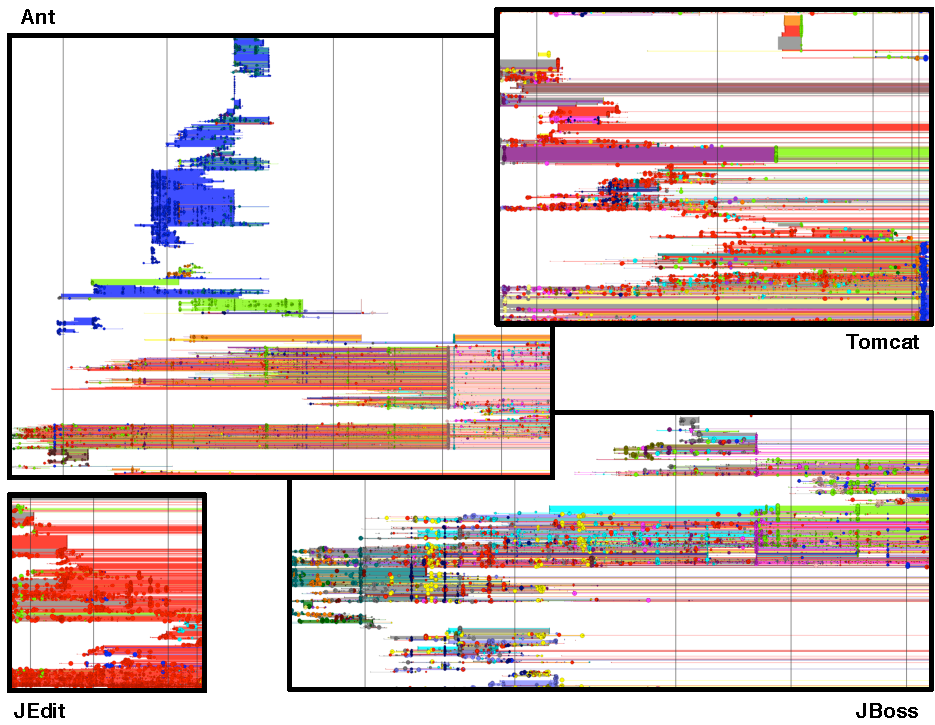
\includegraphics[width=12.5cm]{fig/casestudies-overview.pdf}
\caption{The Ownership Map of Ant, Tomcat, JEdit, and JBoss.}
\label{fig:casestudies-owerview}
\end{center}
\end{figure*}

autoref{fig:casestudy-outsight} shows the \omap of four open-source projects: Ant, Tomcat, JEdit, and JBoss. The views are plotted with the same parameters as the map in the previous case study, the only difference is that vertical lines slice the time axis into periods of twelve instead of three months. Ant has about 4'500 files with 60'000 revisions, Tomcat about 1'250 files and 13'000 revisions, JEdit about 500 files and 11'000 revisions, and JBoss about 2'000 files with 23'000 revisions.

Each view shows a different but common pattern. The paragraphs below discuss each pattern briefly.

\textbf{Ant.} The view is dominated by a huge Expansion. After some time of development, the very same files fall victim to a huge Cleaning. This pattern is found in many open-source projects: Developers start a new side-project and when grown up it moves to an own repository, or the side-project ceases and is removed from the repository. In this case, the spin-off is the Myrmidon project, a ceased development effort planned as successor to Ant.

\textbf{Tomcat.} The colors in this view are, apart from some large blocks of Silence, well mixed. The \omap shows much Dialogue and hotspots with Teamwork. Thus this project has developers that  collaborate well.

\textbf{JEdit.} This view is dominated by one sole developer, making him the driving force behind the project. This pattern is also often found in open-source projects: being the work of a single author that contributed about 80\% of the code.

\textbf{JBoss.} The colors in this view indicate that the team underwent to large fluctuations. We see twice a sudden change in the colors of both commits and code ownership: once mid 2001 and once mid 2003. Both changes are accompanied by Cleanings and Expansions. Thus the composition of the team changed twice significantly, and the new teams restructured the system.

%%%%%%%%%%%%%%%%%%%%%%%%%%%%%%%%%%%%%%%%%%%%%%%%%%%
\section{Discussion}\label{sec:discussion}
%%%%%%%%%%%%%%%%%%%%%%%%%%%%%%%%%%%%%%%%%%%%%%%%%%%

\textbf{On the exploratory nature of the implementation.} We implemented our approach in Chronia, a tool built on top of the Moose reengineering environment \cite{Duca05a}. autoref{fig:chronia} emphasizes the interactive nature of our tool.

On the left of autoref{fig:chronia} we see Chronia visualizing the overall history of the project, which provides a first overview. Since there is too much data we cannot give the reasoning only from this view, thus, Chronia allows for interactive zooming. For example, in the window on the lower right, we see Chronia zoomed into the bottom right part of the original view. Furthermore, when moving the mouse over the \omap, we complement the view by also showing the current position on both time and file axis are highlighted in the lists on the right. These lists show all file names and the timestamps of all commits. As Chronia is build on top of Moose, it makes use of the Moose contextual menus to open detailed views on particular files, modules or authors. For example, in the top right window we see a view with metrics and measurements of a file revision.

\begin{figure*}[htbp]
\begin{center}
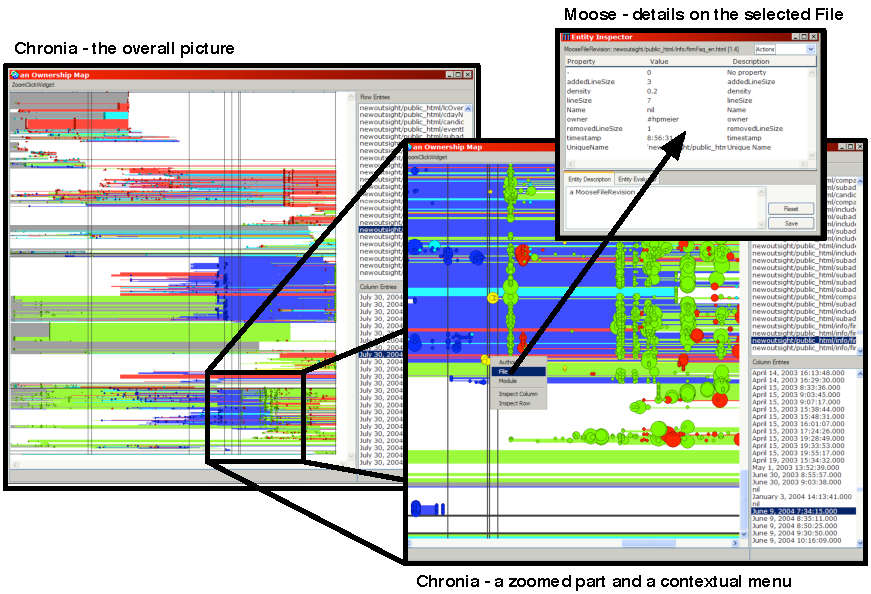
\includegraphics[width=\linewidth]{fig/chronia-screenshot}
\caption{Chronia is an interactive tool.}
\label{fig:chronia}
\end{center}
\end{figure*}

\textbf{On the scalability of the visualization.} Although Chronia provides zooming interaction, one may lose the focus on the interesting project periods. A solution would be to further abstract the time and group commits to versions that cover longer time periods. The same applies to the file axis grouping related files into modules.

\textbf{On the decision to rely on CVS log only.} Our approach relies only on the information from the CVS log without checking out the whole repository. There are two main reasons for that decision.

First, we aim to provide a solution that gives fast results; \eg building the \omap of JBoss takes 7,8 minutes on a regular 3 GHz Pentium 4 machine, including the time spent fetching the CVS log information from the \textit{Apache.org} server.

Second, it is much easier to get access to closed source case studies from industry, when only metainformation is required and not the source code itself. We consider this an advantage of our approach.

\textbf{On the shortcomings of CVS as a versioning system.} As CVS lacks support for true file renaming or moving, this information is not recoverable without time consuming calculations. To move a file, one must remove it and add it later under another name. Our approach identifies the author doing the renaming as the new owner of the file, where in truth she only did rename it. For that reason, renaming directories impacts the computation of code ownership in a way not desired.

\textbf{On the perspective of interpreting the \omap.} In our visualization we sought answers to questions regarding the developers and their behaviors. We analyzed the files from an author perspective point of view, and not from a file perspective of view. Thus the \omap tells the story of the developers and not of the files \eg concerning small commits: subsequent commits by different author to one file do not show up as a hotspot, while a commit by one author across multiple files does. The later being the pattern we termed \textit{Edit}.

Also from a project manager point of view the \omap can give valuable hints. Knowing whether a developer tends more to  Takeover or more to Familiarization is a good indicator to whom the responsibility of subsystem should be given. If a subsystem need rewrites and restructuring the Takeover type is a good choice, otherwise if a subsystem is a good base to be built up on the Familiarization type is a good choice.

But classifications of the authors have to be interpreted in their context. If a developer ly takes over subsystems this does not mean that he has an  character or that he will always tend to Takeovers. In our case study (autoref{fig:casestudy-outsight}) Green's Takeover of \id{S2} in \id{P7} must be seen in the context of the system history: Blue left the team and Green was the original developer of \id{S2}. He would have acted differently if Blue were still in the team.

%%%%%%%%%%%%%%%%%%%%%%%%%%%%%%%%%%%%%%%%%%%%%%%%%%%
\section{Conclusions}\label{sec:conclusions}
%%%%%%%%%%%%%%%%%%%%%%%%%%%%%%%%%%%%%%%%%%%%%%%%%%%

In this chapter we aim to understand how the developers drove the evolution of the system. In particular we ask the following questions:
\begin{itemize}
\item How many authors developed the system?
\item Which author developed which part of the system?
\item What were the behaviors of the developers?
\end{itemize}

To answer them, we define the \omap visualization based on the notion of code ownership. In addition we semantically group files that have a similar \emph{commit signature} leading to a visualization that is not  based on alphabetical ordering of the files but on co-change relationships between the file histories. The \omap helps in answering which authors are knowledgeable in which part of the system and also reveal behavioral patterns. To show the usefulness we implemented the approach and applied it on several case studies. We reported some of the findings and we discussed the benefits and the limitations as we perceived them during the experiments.

In the future, we would like to investigate the application of the approach at other levels of abstractions besides files, and to take into consideration types of changes beyond just the change of a line of code.

%%%%%%%%%%%%%
%%%%%%%%%%%%%
%%%%%%%%%%%%%
%%%%%%%%%%%%%
%%%%%%%%%%%%%
%%%%%%%%%%%%%
%%%%%%%%%%%%%
%%%%%%%%%%%%%

\chapter{Discovery of Experts}
\label{the chapter on bug reports}

\infobox
	{Discovery of experts}
	{Experts that committed to local codebase}
	{Social (established through lexical and historical information)}
	{Fuzzy problem description given as natural language text}

Given current tool support, following up social cues has to be done through the lexical proxy of a persons name. However, often developers are facing a problem where they need help but not know an expert by name. Either because they are not aware that someone from their personal network is actually on expert on that matter, or because they simply do not know an expert on that matter. There is a clear need for establishing a link between fuzzy problem descriptions and experts, such that developers may follow-up social cues that are otherwise out of their reach. 

In this chapter we present an approach to discover experts without having to know their name. Given a problem description, such as a work item or a bug report, we provide an automated means of linking to the person with the expertise on that matter. Our work deals with assigning incoming bug reports to developers, however the techniques that we developed can be used to establish links from any fuzzy problem description to known experts. To model the expertise of developers, we require a recorded history of their submissions to a system's source base. This information can be taken from a version control system. We use lexical information found in those submission to model the developer's expertise. Even though not discussed in the following chapter, that very information could also be used to render \EVOCLOUDS of the developer's expertise and thus to enable discovery of experts through the means of an story telling visualization.

\asteriskasteriskasterisk

For popular software systems, the number of daily submitted bug reports is high. Triaging these incoming reports is a time consuming task. Part of the bug triage is the assignment of a report to a developer with the appropriate expertise. In this chapter, we present an approach to automatically suggest developers who have the appropriate expertise for handling a bug report. We model developer expertise using the vocabulary found in their source code contributions and compare this vocabulary to the vocabulary of bug reports. We evaluate our approach by comparing the suggested experts to the persons who eventually worked on the bug. Using eight years of Eclipse development as a case study, we achieve 33.6\% top-1 precision and 71.0\% top-10 recall.

\todo{Do not forget to remove the page numbers in the camera-ready version!}
Software repositories of large projects are typically accompanied by a bug report tracking system. In the case of popular open source software systems, the bug tracking systems receive an increasing number of reports daily. The task of triaging the incoming reports therefore consumes an increasing amount of time \cite{Anvi06b}. One part of the triage is the assignment of a report to a developer with the appropriate expertise. Since in large open source software systems the developers typically are numerous and distributed, finding a developer with a specific expertise can be a difficult task.

Expertise models of developers can be used to support the assignment of developers to bug reports. It has been proposed that tasks such as bug triage can be improved if an externalized model of each programmer's expertise of the code base is available \cite{Frit07a}. Even though approaches for expertise models based on software repository contributions are available, existing recommendation systems for bug assignment typically use expertise models based on previous bug reports only \cite{Anvi06a,Canf05a,Cubr04b,Mock02b,Lucc02a}.
Typically a classifier is trained with previously assigned bug reports, and is then used to classify and assign new, incoming bug reports.
Our approach differs, we train our recommendations system with all source code contributions up to the reporting date of the bug and then use the bug reports textual description as a search query against the expertise model's \TAM.

In this chapter, we propose an expertise model based on source code contributions and apply in it a recommendation system that assigns developers to bug reports. We compare \VOC found in the \verb$diff$s of a developer's contributions with the vocabulary found in the description of a bug report. We then recommend developers whose contribution vocabulary is lexically similar to the vocabulary of the \BR.

We implemented our approach as a prototype called \DEVLECT\footnote{\DEVLECT is open source, written in Smalltalk, and available at \url{http://smallwiki.unibe.ch/develect}. The name \emph{develect} is a portmanteau word of \emph{developer} and \emph{dialect}. }, and evaluate the recommendation system using the Eclipse project as a case study. We develop and calibrate our approach on a \trainingset of bug reports. Then we report the results of evaluating it on a set of reports of the remaining case study.

The contributions of this chapter are as follows:
\begin{itemize}
\item We propose a novel expertise model of developers. The approach is based on the vocabulary found in the source code contributions of developers.

\item We propose a recommendation system that applies the above expertise model to assign developers to bug reports. We evaluate the system using eight years of Eclipse development as a case study. 

\item We report on the decay of developer expertise, observed when calibrating our approach. We apply two weighting schemes to counter this effect.
\end{itemize}

%-------------------------------------------------------------------------
\section{Our Approach in a Nutshell}\label{sec:nutshell}

\begin{figure}
    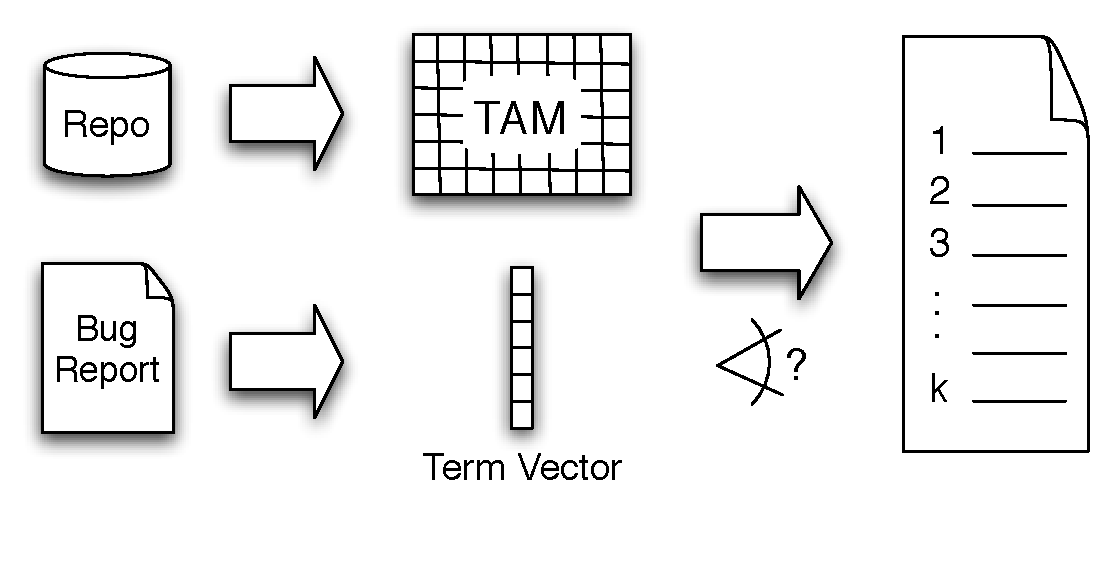
\includegraphics[width=\linewidth]{fig/devlect-pipeline}
    \caption{Architecture of the \DEVLECT recommendation system: (left) bug reports and versioning repositories are processed to produce term vectors and \TAMS; (right) the cosine angle between vector and matrix columns is taken to rank developers in the suggested list of experts.}
    \label{fig:algo}
\end{figure} 

In this chapter we present i) the construction of an expertise model of developers and ii) the application of a recommendation system that uses this expertise model to automatically assign developers to bug reports. Our approach requires a versioning repository to construct the expertise model as well as a bug tracking facility to assign developers to bug reports. We realized the approach as a prototype implementation, called \DEVLECT.

In his work on automatic bug report assignment, John Anvik proposes eight types of information sources to be used by a recommendation system \cite{Anvi06b}. Our recommendation system focuses on three of these types of information: the information of the textual description of the bug (type~1), the one of the developer who owns the associated code (type~6), and the information of the list of developers actively contributing to the project (type~8). We refine information type~6 to take into account the textual content of the code owned by a developer. Our recommendation system is based on an expertise model of the developer's source code contributions. For each developer, we count the textual word frequencies in their change sets. This includes deleted code and context lines, assuming that any kind of change (even deletions) requires developer knowledge and thus familiarity with the vocabulary. 

Our system currently does not consider the component the bug is reported for (type~2), the operation system that the bug occurs on (type~3), the hardware that the bug occurs on (type~4), the version of the software the bug was observed for (type~5), or the current workload of the developers (type~7). Information types 2--4 are indirectly covered, since textual references to the component, operation system, or hardware are taken into account when found in bug reports or source code. Information of type~7 is typically not publicly available for open source projects and thus excluded from our studies. Furthermore, we deliberately disregard information of type~5, since developer knowledge acquired in any version pre-dating the bug report might be of use. 

Given a software system with a versioning repository, the creation of the expertise model works as illustrated in \autoref{fig:algo}:

\begin{enumerate}
\item For each contributor to the versioning repository, we create an empty bag of words. 
\item For each contribution to the versioning repository, we create a \verb$diff$ of all changed files and count the word frequencies in the diff files. We assign the word frequencies to the contributor's bag of words.
\item We create a \TAM $M_{n \times m}$, where $n$ is the global number of words and $m$ the number of contributors. Each entry $m_{i,j}$ equals the frequency of the word $t_i$ in the contributions of the contributor $a_j$. 
\end{enumerate}

Given the above \TAM and a bug tracking facility, the assignment of developers works as follows:

\begin{enumerate}
\item We count the word frequencies in the bug report and create a query vector of length $n$ where $v_i$ equals the frequency of word $t_i$ in the bug report. 
\item For each developer in the \TAM, we take the cosine of the angle between the query vector and the developer's column of the matrix.
\item We rank all developers by their lexical similarity and suggest the top $k$ developers.
\end{enumerate}

To evaluate our approach we use Eclipse as a case study. We train our system with weekly summaries of all CVS commits from 2001 to 2008, and use the resulting expertise-model to assign developers to bug reports. We evaluate precision and recall of our approach by comparing the suggested developers to the persons who eventually worked on the bug and its report.

For example, for a report that was submitted in May 2005, we would train our system with all commits up to April. Then we would evaluate the suggested developers against those persons who worked on the bug and its report in May or later on to see if they match.

 

\section{The Develect Expertise Model}\label{sec:algorithm}

Given the natural language description of a bug report, we aim to find the developer with the best expertise regarding the content of the bug report. For this purpose, we model developer expertise using their source code contributions. 

Developers gain expertise by either writing new source code or working on existing source code. Therefore we use the vocabulary of source code contributions to quantify the expertise of developers. Whenever a developer writes new source code or works on existing source code, the vocabulary of mutated lines (and surrounding lines) are added to the expertise model. These lines are extracted from the \VCS using the \verb$diff$ command.

Natural language documents differ from source code in their structure and grammar, thus we treat both kind of documents as unstructured bags of words. We use Information Retrieval techniques to match the word frequencies in bug reports to the word frequencies in source code. This requires that developers use meaningful names \eg for variables and methods, which is the case given modern naming conventions~\cite{Kuhn07a}. 

Given a bug report, we rank the developers by their expertise regarding the bug report. The expertise of a developer is given by the lexical similarity of his vocabulary to the content of the bug report.

\subsection{Extracting the Vocabulary of Developers from Version Control}

To extract the vocabulary of a specific developer we must know which parts of the source code have been authored by which developer. 
%read and changed by this developer !!!

We extract the vocabulary in two steps, first building a \textsc{Chronia} model of the entire repository \cite{Girb05c} and then collecting word frequencies from the \verb$diff$ of each revisions. %Depending on the particular versioning system, it can require an additional effort to identify revisions. For example, in CVS version numbers are associated with single files instead of the entire repository.
The \verb$diff$ command provides a line-by-line summary of the changes between two versions of the same file. The diff of a revision summarizes the changes made to all files that changed in that revision of the repository. The identifier names and comments that appear on these lines give us evidence of the contributor's expertise in the system. Thus, we add the word frequencies in a revision's \verb$diff$ to the expertise model of the contributing developer.

Word frequencies are extracted as follows: the lines are split into sequences of letters, which are further split at adjacent lower- and uppercase letters to accommodate the common \emph{camel case} naming convention. Next stopwords are removed (\ie common words such as \emph{the}, \emph{and}, etc). Eventually stemming %\cite{Port80a}
is applied to remove the grammatical suffix of words.

The comment message associated with a revision is processed in the same way, and added to the expertise model of the contributing developer as well. 
%This is done on a per file basis: the comment message of a commit including many files is weighted higher than the comment message of a single file commit.

%\todo{Add conclusional paragraph which sums up this subsection}

\subsection{Modeling the Expertise of Developers as a Term-Author-Matrix}

We store the expertise model in a matrix that correlates word frequencies with developers. We refer to this matrix as a \TAM. Although, technically it is a term-document-matrix where the documents are developers. (It is common in Information Retrieval to describe documents as bags of words, thus our model is essentially the same, with developers standing in for documents.)

The \TAM has dimension $n \times m$, where $n$ is the global number of words and $m$ the number of contributors, that is developers. Each entry $m_{i,j}$ equals the frequencies of the word $t_i$ summed up over all source code contributions provided by developer $a_j$.
%Furthermore, we weight the matrix with \emph{tf-idf} (term frequencyinverse document frequency) to balance rare and common words.

We have found that results improve if the \TAM is weighted as follows:

\begin{itemize}
\item \emph{Decay of Vocabulary.} For each revision, the word frequencies are weighted by a decay factor that is proportional to the age of the revision. In the Eclipse case study, best results are obtained with a weighting of $3\%$ per week (which accumulates to $50\%$ per half year and $80\%$ per annum). Please refer to \autoref{sec:discussion} for a detailed discussion.
\end{itemize}

\subsection{Assign Developers to Bug Reports regarding their Expertise}

To assign developers to bug reports, we use the bug report's textual content as a search query to the \TAM.
%Our current tool supports the extraction of bug reports from Bugzilla, however our approach works with any textual representation of bug reports, even with raw text.
Given a Bugzilla\footnote{http://www.bugzilla.org} bug report, we count the word frequencies in its textual content. In particular we process both short and all long descriptions (threats to validity see \autoref{sec:discussion}).
\todo{ XXX, mail this to migod! }
We disregard attachments that are Base-64 encoded, such as attached images, as well as fields that refer to persons. From the extracted word frequencies, we create a \emph{term vector} that uses the same word indices as the \TAM. % The lexical similarity between term vectors is obtained using the cosine between both vectors.
We then compute the lexical similarity between two term vectors by taking the cosine of the angle between them.
The similarity values range from $1.0$ for identical vectors to $0.0$ for vectors without shared terms. (Negative similarity values are not possible, since word-frequencies cannot be negative either.)

We compare the term vector of the bug report with the term vectors of all developers (\ie the columns of the \TAM) and create a ranking of developers. For the assignment of bug reports to developers, a suggestion list of the top-$k$ developers with the highest lexical similarities is then provided.

We have found that the results improve if the \TAM is further weighted as follows:
\begin{itemize}
\item \emph{Inactive Developer Penalty.} If a developer has been inactive for more than three months, the lexical similarity is decreased by a penalty proportional to the time since his latest contribution. In the Eclipse case study, best results are obtained with a penalty of $0.2$ per annum. Please refer to \autoref{sec:discussion} for a detailed discussion.
\end{itemize}

\section{Case Study: \EC platform}\label{sec:casestudy}

To evaluate our approach we take Eclipse\footnote{http://www.eclipse.org/eclipse} as a case study. \EC is a large open source software project with numerous active developers.
\EC has been developed over several years now. Therefore, its version repository contains a great deal of source code developed by many different authors.
% a lot of source code of different authors can be obtained from its versioning system CVS.
Furthermore, \EC uses Bugzilla as its bug tracking system, storing \BRs dating back to nearly the beginning of the project.
% where \BRs dated from today until almost the beginning of the development are stored.
%These circumstances make \EC a project well suited to extract large \VOC data of many different authors from and to query that data with also from \EC extracted \BRs. Since such a query should yield the author with the best expertise regarding the bug report,
We evaluate our results by comparing the top-$k$ developers with the persons who eventually worked on the bug report.

Our case study covers the Eclipse project between April 22, 2001, and November 9, 2008. The source code contributions of Eclipse are stored in a CVS repository\footnote{:pserver:anonymous@dev.eclipse.org/cvsroot/eclipse}, the bug reports in a Bugzilla database\footnote{https://bugs.eclipse.org/bugs}. This represents almost eight years of development, including 130,769 bug reports and 162,942 global revisions (obtained from CVS's file versions using a sliding time-window of 2 minutes \cite{Zimm04a}). During this time, 210 developers contributed to the project.

\subsection{Setup of the Case Study}

The setup of the Eclipse case study consists of two different parts. The first part is about the change database, here we use all changes before the actual bug report. The second part is about the bug database, here we make 10 partitions of which two are used in this case study. We process and evaluate  both parts in weekly iterations as follows:
\begin{itemize}
\item We create a \DEVLECT expertise model based on contributions between April 22, 2001, and the last day of the previous week.
\item We generate a suggested list of the top-10 experts for all bug reports submitted in the current week.
\item We evaluate precision and recall by comparing the suggestion list with the developers who, between the first day of the next week and November 9, 2008, eventually worked on the bug report.
\end{itemize}

For example, for a bug report submitted on May 21, 2005, we would train our system with all commits between April 22, 2001 and May 15, 2005, and then evaluate the list of suggested experts against the set of developers who, between May 23, 2005, and November 9, 2008, eventually handled the bug report.

We use systematic sampling to create 10 partitions of 13,077 bug reports (ordered by time) that span the entire time of the project. One partition is used as \trainingset for the development of our approach, and another partition is used as \validationset to validate our approach. We applied the approach to the \validationset only after all implementation details and all calibration parameters had been finally decided on. The other partitions remain untouched for use as \validationset in future work.

In this section, we report on our results obtained on the validation partition \#2. In \autoref{sec:discussion} we report on results obtained from the training partition \#1 while calibrating the approach.

%We developed and calibrated our approach on just the first partition. Only after all implementation details and all calibration parameters had been finally decided on, did we apply the approach to the remaining partitions.

%\subsection{Settings of the Case Study}

%The results of the evaluation in this section are obtained by running \DEVLECT with the following settings:
%{\footnotesize \begin{verbatim}
%  project = Eclipse
%  stemming = Porter
%  scanner = CamelCaseScanner
%  stopwords = English
%  similarity = Cosine
%  TAM weighting = None
%  use LSI = false
%  added lines weighting = 1.0
%  removed lines weighting = 1.0
%  context lines weighting = 1.0
%  comments weighting = 1.0
%  decay of vocabulary (per week) = 0.97
%  inactive developer penalty (per annum) = 0.2
%  excluded fields = Persons, Base64
%  weekly diffs = true
%  co-developer weighting = Sqrt
%  start date = 2001-04-22
%  end date = 2008-11-02
%  exclude unmapped logins = true
%  partition (1->validation, else->test) = 2
%\end{verbatim}}

\subsection{Precision and Recall}

We evaluate our approach by comparing the suggested list of experts with the developers who eventually worked on the bug report. We report on precision and recall for different sizes of suggested lists, between $k = 1$ and $k = 10$. Comparing our results to the persons who eventually worked on the bug is not optimal. For example, the person could have been assigned to the bug report by some factor other than expertise. Obtaining a better list of experts requires manual interrogation of the development team.

Precision is the percentage of suggested developers who actually worked on the bug report. Recall is the percentage of developers who worked on the bug who were actually suggested. It is typical for Information Retrieval approaches that there is a trade-off between precision and recall.

Getting the list of persons who eventually worked on a bug report is tricky. The \emph{assigned-to} field does not always denote a person who eventually solved the bug report \cite{Cubr04b, Anvi06a, Anvik07}. Therefore we compare our results against three configurations (C1--C3) of bug-related persons:

\begin{enumerate}
\item Developers who committed an actual bug fix to the software repository. For \EC, this information is not stored in the Bugzilla database, therefore we must rely on information from CVS commit messages. In the \validationset, this information is provided for 14.3\% of the bug reports only. This configuration evaluates how well we perform in suggesting experts who provide actual bug fixes.
\item Persons given by the \emph{assigned-to} field or a \emph{who} field of the bug report. That is, the eventual assignee (if this is a developer) and all developers who ever discussed the bug in the comment section of the report. This configuration evaluates how well we perform in suggesting experts who are capable of understanding and discussing the bug. Note that resolving a bug is not limited to providing code fixes; often the discussion is just as important to the resolution of the bug. 
\item As in configuration \#2, but additionally including the person identified by the \emph{reporter} field, if the reporter is a developer, \ie has a CVS login. \todo{check last comment} This reflects the fact that bugs are sometimes resolved by the same people who find and track them.
\end{enumerate}

Please refer to \autoref{sec:discussion} for further discussion of the above configurations and their threats to validity.

\subsection{Results}\label{therealthing}

\begin{figure}
    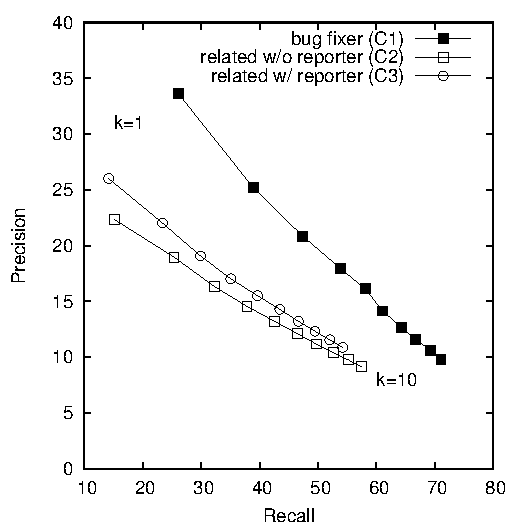
\includegraphics[width=\linewidth]{fig/devlect-test-set}
    \caption{Recall and precision of the Eclipse case study: configuration C1 scores best with $33.6\%$ top-1 precision and $71.0\%$ top-10 recall.}
    \label{fig:eclipse}
\end{figure} 

\autoref{fig:eclipse} illustrates the results of the Eclipse case study. We compare lists of suggested persons of list size 1 to 10 with set of ``bug related persons'' as given by the three configurations (C1-3) above.

The figure illustrates that recall and precision of configuration C1 are better than C2 and C3. When comparing the suggested list to the bug fixing person~(C1) we achieved the best score with 33.6\% top-1 precision only and 71.0\% top-10 recall. Comparing of the suggested list to all related persons~(C3) we score 26.0\% top-1 precision and 54.2\% top-10 recall. When excluding the reporter of the bug report~(C2) from the suggested list scores are at 22.3\% top-1 precision and 57.4\% top-10 recall.

The fact that configuration C3 scores slightly better then C2 indicates that bug reporters are sometimes indeed experts regarding the reported bug and thus should be considered when triaging bug reports. We can thus conclude that an automatic assignment system should provide to the triaging person a suggested list of people that may include the reporter.

\section{Discussion}\label{sec:discussion}

In this section, we first discuss the calibration of our approach and then cover threats to validity.

Compared to related work, an advantage of our approach is that we do not require a record of previous \BRs. We are able to recommend developers who did not work on bugs previously. For example, we do not require that developers have worked on at least 10 resolved bug reports. On the other hand, our approach requires at least a half to one year of versioning history in order to suggest developers. 

One obvious threat to validity is the quality of our evaluation benchmark. We compare our suggested list against the developers who eventually worked on the bug report and assume that these are the top experts. For example, the bug report could have been assigned to a developer by some factor other than expertise. This threat is hard to counter. A better list of experts can be obtained by manual interrogation of the development team, but even this is not a golden oracle.

Another threat to validity is that we use all long descriptions, including comments, of a bug report as information source. This may include discussions that happened after the bug has been eventually assigned or fixed, information which is not actually available when doing initial bug triage. This might impact the performance of our approach. 


\begin{figure*}
    \center
    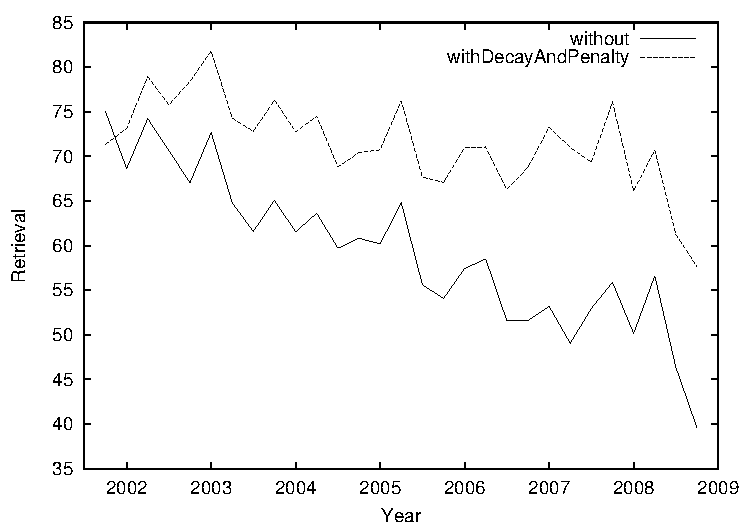
\includegraphics[width=0.40\linewidth]{fig/devlect-graph-left}
    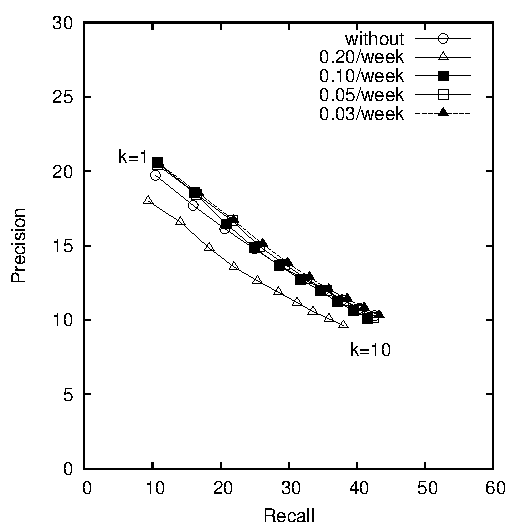
\includegraphics[width=0.28\linewidth]{fig/devlect-graph-middle}
    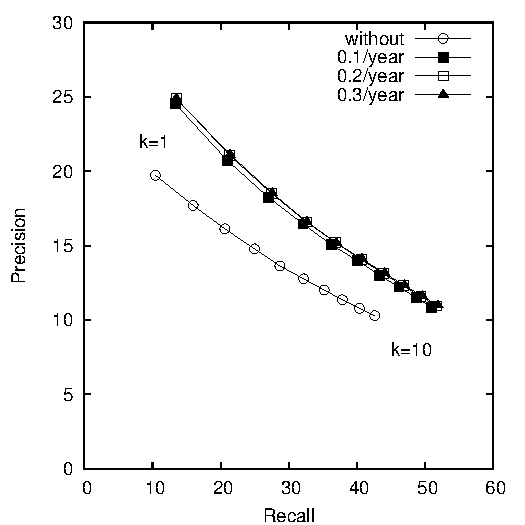
\includegraphics[width=0.28\linewidth]{fig/devlect-graph-right}
    \caption{Decay of vocabulary: (left) decreasing quality of unweighted results, compared to results with \emph{decay of vocabulary} and \emph{inactive developer penalty} settings, (middle) precision and recall for different decay of vocabulary settings, (right) precision and recall for different inactive developer penalty settings.}
    \label{fig:decay}
\end{figure*} 

\subsection{On the Calibration of \DEVLECT}

We used 1/10th of the Eclipse case study as a \trainingset to calibrate our approach. The calibration results are summarized in \autoref{thetable}.

The table lists top-1 precision and top-10 recall. On the first row, we list the results before calibration $(p = 19.7\%, r = 42.6\%)$, and on the last row the results of the final calibration. Please note that the final results on the \trainingset are slightly better than the results reported in \autoref{therealthing} for the \validationset.

\begin{table}
\center
{\footnotesize \begin{tabular}{l | c  c}
  Settings & Precision & Recall \\ \hline
  reference & 19.7 & 42.6 \\ 
  weighted \verb$diff$ & 18.5 & 41.1 \\
  desc. fields only & 16.7 & 37.7 \\
  with LSI & 16.5 & 35.1 \\
  decay 0.03 & 20.5 & 43.2 \\ 
  decay 0.05 & 20.4 & 42.4 \\ 
  decay 0.10 & 20.5 & 41.5 \\ 
  decay 0.20 & 18.0 & 38.0 \\ 
  penalty 0.1 & 24.5 & 50.9 \\ 
  penalty 0.2 & 24.8 & 51.6 \\ 
  penalty 0.3 & 24.8 & 51.9 \\
  final calibration & 26.2 & 54.6 \\
\end{tabular}
}\vspace{0.1in}
\caption{Summary of calibration of \trainingset, for each settings top-1 precision and top-10 recall are given.}
\label{thetable}
\end{table}

The output of the \verb$diff$ command consists of added, removed, and context lines. We experimented with different weightings for these lines (weighted \verb$diff$ in Table 1% 
%\autoref{thetable}
). However, we found that weighting all lines the same yields best results. 

As Bugzilla bug reports consist of many fields, we experimented with different selections of fields. We found that taking short and long descriptions (``desc. fields only'' in \autoref{thetable}) yields worse results than selecting all fields except those that refer to persons, or Base64 encoded attachments. 

We also experimented with Latent Semantic Indexing (LSI), an Information Retrieval technique typically used in search engines that detects polysemy and synonymy by statistical means~\cite{Deer90a}. However, we found that LSI yields poor results (``with LSI'' in \autoref{thetable}).

\subsection{On the Decay of Vocabulary}

In our experiments, we found that developer expertise decays over time. In our approach we introduced two weighting schemes to counter this effect: 

\begin{itemize}
\item \emph{Decay of Vocabulary.} For each revision, the word frequencies are weighted by a decay factor that is proportional to the age of the revision. Developers change their interests and by doing so change their expertise and \VOC. To take such a shift into account, we fade the old \VOC out bit by bit every week, so that the newest words are weighted slightly more than older ones. With time, the old words eventually fade out completely.
\item \emph{Inactive Developer Penalty.} If a developer has been inactive for more than three months, the lexical similarity is decreased by a penalty proportional to the time since his latest contribution to the software system. Inactive developers will most likely not resolve bugs anymore. In order to only recommend currently active developers (we assign \BRs during a period of eight years), developers who did not recently make a change to the software system receive a penalty.
%This penalty consists either of raising the distance to a \BR to assign (depending on the days since their last change) or of downgrading the rank in the list of the authors (ordered by distance).
\end{itemize}

\noindent \autoref{fig:decay} illustrates the effect of these settings. On the left, the unbroken curve illustrates the decreasing quality of unweighted results, whereas the dotted curve shows the results obtained with weighting. Even though results improved significantly, the quality of the weighted results still slightly decreases over time. We cannot fully explain this effect; it may be due to the increasing complexity of \EC as a project, or perhaps the lack of mappings from CVS logins to persons (see \autoref{sec:scvmapping}) in the early years of the project impacts the results. Another cause for the trend in the most recent year, \ie 2008, might be that the list of persons that worked on a bug is not yet completely known to us, which may impact the evaluation.


In the middle of \autoref{fig:decay}, precision and recall for different \emph{decay of vocabulary} settings are given. On the right, precision and recall for different \emph{inactive developer penalty} settings are given. 

Decay of vocabulary scores best results with a weighting of $3\%$ per week (which accumulates to $50\%$ per half year and $80\%$ per annum). This shows that implementation expertise acquired one year ago or earlier does not help in assigning developers to bug reports.

The inactive developer setting scores best results with a penalty of $0.2$ per annum. As a result of the penalty, the matching score of a developer who has been inactive for a year is decreased. The matching scores are the lexical similarity values (between 1.0 and 0.0). Decreasing this value by 0.1 or more is typically enough to exclude a result from the top-10 list. 

Interestingly, any penalty above 0.1 is better than none. The results obtained with different penalty values are almost the same. Please note, that even though the penalty removes inactive developers from the top of the suggested list, their vocabulary is not lost. The results reported for the calibration of the penalty do not make use of vocabulary decay. If a developer becomes active again, all his past expertise is reactivated as well. Thus, we use a moderate penalty of 0.2 in combination with a decay of 3\% as the final calibration settings.

\subsection{On Grouping Diffs by Week}

To cope with the size of our case study, we decided to run weekly iterations rather than fine-grained iterations per bug report and revision. This reduced the time complexity from over 160,000 iterations down to 394 weekly iterations.

Grouping diffs by both author \emph{and} week introduces the following threats to validity: 
If \VOC is added and removed within the same week, it does not add to the developer's expertise. 
In the same way, if a file is added and removed within the same week, it is not taken into account at all. 
If bug reports are submitted late in the week, we might miss developers who acquired novel expertise early in the week. 

If several authors worked on the same file, we cannot tell their weekly contributions apart. In this case, we weight the word frequencies by $\frac{1}{\sqrt{n}}$, where $n$ is the number of co-developers, and assign the weighted frequencies to all co-developers. For the \EC case study, this applies to 3.6\% of weekly file changes.

\subsection{On other Threats to Validity}\label{sec:scvmapping}

% the golden oracle of experts is never available.

Establishing an identity relationship between CVS logins and people mentioned in \BRs is not trivial. The developer information in the CVS log is provided as a mere login name. People mentioned in a Bugzilla \BR are listed with their email address and sometimes additionally with their first and last name. For \EC, the mapping between logins and active developers can be found on the \EC website\footnote{http://www.eclipse.org/projects/lists.php}. However, the list of names of the former \EC developers does not include their corresponding logins\footnote{http://www.eclipse.org/projects/committers-alumni.php}. We could not map 17.1\% of the CVS logins and had thus to exclude 2.7\% of the bug reports from our evaluation.   

Information about copy patterns is not available in CVS. Bulk renaming of files appears in the change history of CVS as bulk removal of files followed by bulk addition of files. Given our current implementation of \DEVLECT, this may lead to an incorrect acquisition of developer knowledge, since the entire vocabulary of the moved files is assigned to the developer who moved the files.
We are thus in good shape to further improve our results by using a copy pattern detection approach~\cite{Chan08a}.

\section{Conclusion}\label{sec:eventually}

We presented a novel expertise model of developers. The model is based on the source code vocabulary of developers. The vocabulary of developers is obtained from the \verb$diff$ of their source code contributions. We applied the model in a recommendation system that assigns developers to bug reports. We evaluated the recommendation system using eight years of Eclipse development as a case study, and achieved 33.6\% top-1 precision and 71.0\% top-10 recall. 

When calibrating our approach, we found that developer expertise decays over time. To counter this effect we applied two weighting schemes: i) \emph{decay of vocabulary} weights expertise by a decay factor that is proportional to the time since the developer acquired that expertise, ii) \emph{inactive developer penalty} downgrades developers that had been inactive for a certain time.

In the future, we would like to extend our expertise model with developer knowledge from other sources, \eg mailing lists. Furthermore we would like to include additional Information Retrieval techniques, as well as combine our approach with approaches that are trained on previous bug reports (\eg \cite{Anvi06a, Canf05a, Cubr04b, Lucc02a}).

For more information on \DEVLECT and the case study presented in this chapter, please refer to the Master's thesis of Dominique Matter \cite{Matt09a}.


%%%%%%%%%%%%%
%%%%%%%%%%%%%
%%%%%%%%%%%%%
%%%%%%%%%%%%%
%%%%%%%%%%%%%
%%%%%%%%%%%%%
%%%%%%%%%%%%%
%%%%%%%%%%%%%

\chapter{Credibility of Code-Search}
\label{the chapter on codesearch}

\infobox
	{Discovery of trustworthy projects}
	{Open-source projects on the internet}
	{Episodic (established through social and historical information)}
	{Name of an open-source project}

Searching for code examples or libraries on the internet is a common code orientation task. Developers do use code search engines to discover source code that they need in order to answer a technical question, such as implementing a given functionality. In interviews with developers, we have found that credibility is one of the major issues when copying source code from an external and thus untrusted source such as the internet. Other than internal sources, code examples taken from external source are possibly written by an untrusted author.

We found that developer follow-up social cues rather than technical issues in order to asses the trustworthiness of code search results. On a second thought, this is not surprising: when developers copy-paste code, they do because they either do not have the time or do not have the expertise to technically understand the problem, thus assessing trustworthiness based on social cues as a pragmatic alternative---given the assumption that more trustworthy developers do write more trustworthy source code. For example, we have found that developers are more likely to assess a search result as trustworthy if it has been written by an author they do know or by an author that belongs to a company or to an open source project that they do value for its credibility. Automating this process may help the reduce the time and effort that developers have to spend on following-up social cues related to code search results.

\asteriskasteriskasterisk

The promise of search-driven development is that developers will save time and resources by reusing external code in their local projects. To efficiently integrate this code, users must be able to trust it, thus \emph{credibility} of code search results is just as important as their relevance. 
%
In this chapter, we introduce a \emph{credibility metric} to help users assess the trustworthiness of code search results and therefore ease the cost-benefit analysis they undertake trying to find suitable integration candidates. The proposed credibility metric incorporates both user votes and cross-project activity of developers to calculate a \emph{``karma''} value for each developer. Through the karma value of all its developers a project is ranked on a credibility scale.
%
We present \Jbd, a proof-of-concept code search engine which implements our credibility metric and we discuss preliminary results from an evaluation of the prototype.

Code search engines help developers to find and reuse software. However, to support search-driven development it is not sufficient to implement a mere full text search over a base of source code, human factors have to be taken into account as well. At last year's SUITE workshop \cite{Kuhn09a}, \emph{suitability} and \emph{credibility} have been major issues in search-driven development, besides---of course---relevance of search results.  

In this chapter we focus on the \emph{credibility} of search results. Relevance of code search results is of course paramount, but credibility in the results is just as important. Before integrating a search result the developer has to assess its trustworthiness to take a go-or-no-go decision. A well-designed search interface allows its users to take this decision on the spot. Gallardo-Valencia \etal found that developers often look into human rather than technical factors to assess the credibility of search results \cite{Gall09a}. For example developers will prefer results from well-known open source projects over results from less popular projects.

In this chapter we present a credibility metric for search results. The credibility metric is based on human factors. We use data collected from Web 2.0 platforms to assess the trustworthiness of both projects and developers. Our credibility metric is based on collaborative filtering of user votes and cross-project activity of developers. For example, if a little-known project is written by developers who also contributed to a popular open source project, the little-known project is considered to be as trustworthy as the popular project. 

As a feasibility study, we implemented the credibility metric in \Jbd, a proof-of-concept code search engine. The index of our \Jbd installation currently contains credibility assessments for over 3,700 projects, based on 193,000 user votes and the cross-project activity of over 56,000 developers. In this chapter, preliminary results from an evaluation of the prototype are discussed.

Contributions of this chapter are as follows.
\begin{itemize}
\item We introduce a credibility metric for software projects. The credibility metric is based on human factors, and uses collaborative filtering of both user votes and cross-project activity of developers.
\item We present \Jbd, a proof-of-concept implementation of our credibility metric and discuss preliminary results from an evaluation of the prototype.
\end{itemize}

% =====================================================================
\begin{figure}
  \centering
    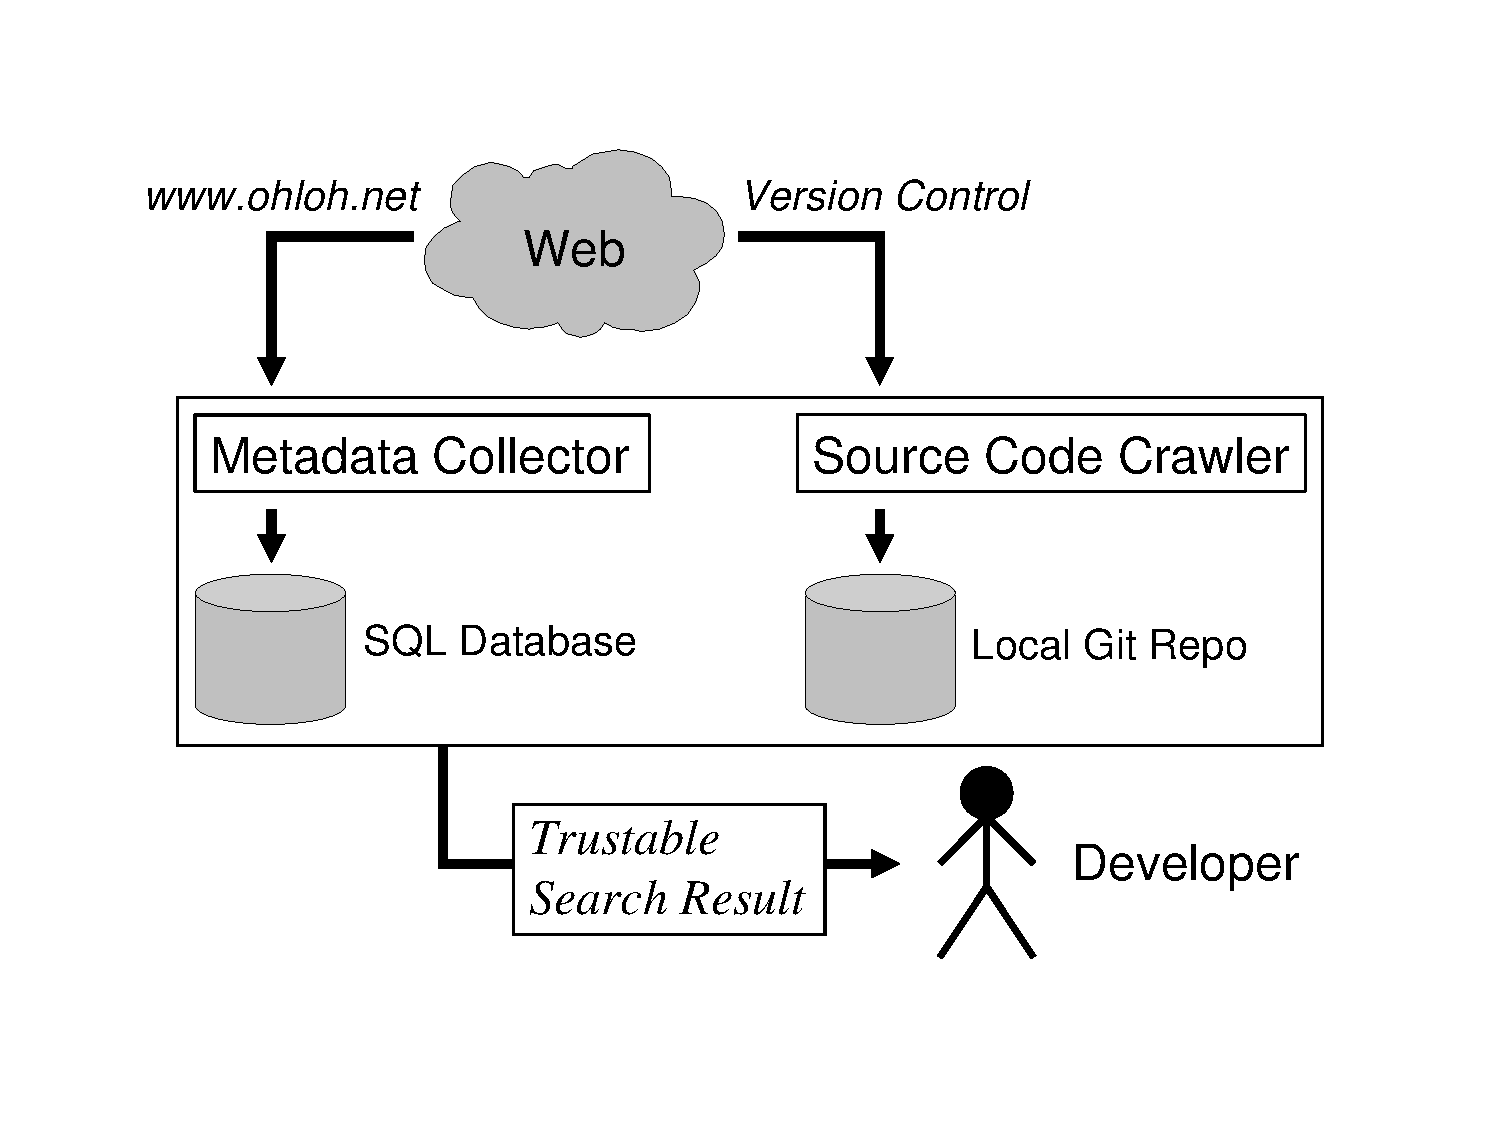
\includegraphics[width=\linewidth]{fig/bender-architecture-diagram}
    \caption{
    {\small
    Architecture of the \Jbd prototype. \Jbd enhances search results from source code with a credibility estimate that is based on social data collect from the Ohloh Web 2.0 website.
    }
    }
    \label{fig:archi}
\end{figure}
% =====================================================================
\section{Credibility Metric}
\label{sec:metric}

\begin{figure*}
  \centering
  	 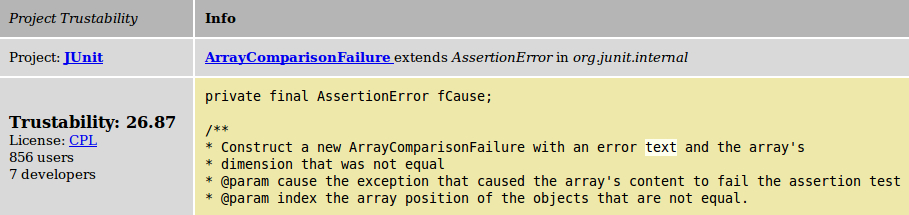
\includegraphics[width=\linewidth]{fig/bender-screenshot}
    \caption{
    {\small
    Screenshot of a \Jbd search result with credibility estimate. On the right there is the actual search result, with full name and code snippet. On the left there is information about the originating project and the trust value calculated by the credibility metric.
    }
    }
    \label{fig:screenshot}
\end{figure*}

In this section, we propose a credibility metric for code search results that uses collaborative filtering of both user votes and cross-project activity of developers.

To assess the credibility of code search results we combine traditional full text search with meta-information from Web 2.0 platforms. Our credibility metric requires the following information:

\begin{itemize}
\item A matrix $M = (c_{d,p})$ with the number of contributions per contributor $d$ to a project $p$.
\item A vector $V = (v_p)$ with user votes for software projects to signal the users' trust in projects. Gallardo-Valencia \etal refer to user votes as ``fellow users'' \cite{Gall09a}.
\end{itemize}

We use collaborative filtering of both user votes and cross-project activity of developers. For example, if a little-known project is written by developers who have also contributed to a popular open source project, the little-known project is considered to be as trustable as the popular project. Since both the number of contributions per contributor and the number of votes per project follow a power-law distribution, we use \emph{log} weighting and \emph{tf-idf}\footnote{``term frequency-inverse document frequency'' \url{http://en.wikipedia.org/wiki/Tf-idf}} weighting where applicable. 

First we define the \emph{karma} of a contributor as

    $$K_{d} = \sum_{P} w_{d,p} \log v_p
    \quad \mathrm{where} \quad 
    w_{d,p} = \frac{\log c_{d,p}}{\log \mathrm{df}(d)}$$

\noindent
which is the sum of the votes of all projects, weighted by the number of contributions to these projects and divided by the inverse project frequency of the contributor (\ie the number of projects to which the contributor contributed at least one contribution).


Based on this, credibility of a project is defined as 

	$$T_{p} = \sum_{D} w_{d,p} K_d
	\quad \mathrm{where} \quad 
	w_{d,p} = \frac{\log c_{d,p}}{\sum_{d' \in D} \log c_{d',p}}$$

\noindent
which represents the sum of the karma of all the projects contributors, weighted by the number of their contributions.
Note that we divide project credibility by the total number of contributions, but not contributor karma. This is on purpose, contributors are more trustable the more they commit (based on the assumption that all accepted commits require approval of a trusted core developer, as is common in many open source projects) but projects are not per se more trustable the larger they are.

To summarize, we consider a project to be trustable if there are significant contributions by contributors who have also significantly contributed to projects (including the project in question) that have received a high number of user votes.

The proposed definition of credibility is dominated by cross-project contributors, \ie contributors who contributed many times to many projects with many votes. This is in accordance with empirical findings on open source that have shown how cross-project developers are a good indicator of project success \cite{Kats07a}. This behaviour is also known as ``the rich get richer'' in the theory of scale-free networks and is considered an inherent and thus common property of most social networks \cite{Bara03a}.

% =====================================================================
\section{The JBender Prototype}
\label{sec:approach}

We have developed a prototype, called \Jbd, which enriches code search results with credibility information. To add to the information content of search results we combine two main sources to form the \Jbd code search engine. On the one hand there is the actual code base of the search engine over which an index is created. On the other hand we have created a database of metadata for the projects in the code base. 

\autoref{fig:archi} illustrates the architecture of \Jbd. \Jbd creates a searchable index over the code base and provides a code search over it. Its novelty however lies in the underlying metadata which is linked to the projects in the searchable code base - upon finding results from the latter \Jbd can supply the meta information stored for the result's originating project.


\begin{figure*}
{\small
  \centering
\begin{tabular}{ l | l | l }%{ | l || l || l |}
%\hline
%% row 1
\textbf{Top projects (by votes)} & \textbf{Top Developer (by karma)} & \textbf{Top projects (by credibility)}
\\\hline
%% row 2
``firefox", $v_p$ = 7207 & ``darins", $K_{d}$ = 71.97 & ``grepWin", $T_{p}$ = 51.60, $v_p$ = 32
\\%\hline
%% row 3
``subversion", $v_p$ = 5687 & ``amodra", $K_{d}$ = 70.11 & ``GNU Diff Utilities", $T_{p}$ = 51.18, $v_p$ = 645
\\%\hline
%% row 4
``apache", $v_p$ = 5107 & ``darin", $K_{d}$ = 69.09 & ``Eclipse Ant Plugin", $T_{p}$ = 49.76, $v_p$ = 136
\\%\hline
%% row 5
``mysql", $v_p$ = 4834 & ``nickc", $K_{d}$ = 67.14 & ``Eclipse Java Development Tools", $T_{p}$ = 48.36, $v_p$ = 647
\\%\hline
%% row 6
``php", $v_p$ = 4081 & ``Dani Megert", $K_{d}$ = 66.51 & ``Crimson", $T_{p}$ = 42.41, $v_p$ = 2
\\%\hline
%% row 7
``openoffice", $v_p$ = 3118 & ``mlaurent", $K_{d}$ = 66.14 & ``GNU binutils", $T_{p}$ = 42.18, $v_p$ = 525
\\%\hline
%% row 8
``firebug", $v_p$ = 3109 & ``Paul Eggert", $K_{d}$ = 65.89 & ``syrep", $T_{p}$ = 42.12, $v_p$ = 2
\\%\hline
%% row 9
``gcc", $v_p$ = 2586 & ``kazu", $K_{d}$ = 65.78 & ``GNU M4", $T_{p}$ = 41.85, $v_p$ = 54
\\%\hline
%% row 10
``putty", $v_p$ = 2519 & ``rth", $K_{d}$ = 65.25 & ``gzip", $T_{p}$ = 41.61, $v_p$ = 261
\\%\hline
%% row 11
``phpmyadmin", $v_p$ = 2412 & ``hjl", $K_{d}$ = 65.04 & ``Forgotten Edge OpenZIS", $T_{p}$ = 40.86, $v_p$ = 1
\\%\hline
\end{tabular}
\caption{
{\small
Top ten results for A) project ranking by Ohloh, B) karma of developers, C) project ranking by trustabilty.
}}
\label{fig:table}
}
\end{figure*}

\subsection{JBender's Metadatabase}
Our source of meta data is the \textsc{Ohloh}\footnote{\url{http://www.ohloh.net}} project. Ohloh is a social networking platform for open source software projects where projects (or rather their developers) can specify additional information. However Ohloh does not allow users to actually search through or interact with the source code: Ohloh is not a code search engine. Ohloh provides user contributed information on both open source projects and their developers, composing valuable information for search users. Users can vote for both projects and developers whether and how much they like them by rating projects and giving kudos to certain developers. Furthermore kudos are (automatically) given to developers who have worked for successful projects, i.e. projects with large user bases. 

For the \Jbd prototype we collected the credibility meta-information from Ohloh, which is a social web platform for open source projects that provides user contributed information on both open source projects and their developers.

Metadata stored in the database includes (among others): Description of original project, project homepage, rating of the project, list of current repositories (type, url, last time of update, ...), licenses of files in the project (exact type of license, number of files), employed programming languages (percentage of total, lines of code, comment ratio, ...), the project's users and developers who worked on the project (kudos, experience, commits per project, ...).

\subsection{JBender's Codebase}
In addition to the collected metadata, \Jbd also follows the links to the version control repositories that are listed on Ohloh, creates local copies of these repositories and parses the code in Java projects to build an search index over them.
\Jbd then provides a basic structured code search over various parts of the indexed source code. Examples are method/class names and their bodies, comments, visibility, dependencies and implemented interfaces.

\subsection{credibility enhanced results}

The following data from Ohloh was directly used for the credibility metric: As contributors we used the developers of the projects and as the number of contributions we used the number of commits. As user votes we used the number of developers who ``stacked'' a project, which is Ohloh's terminology for claiming to be an active user of a project.\footnote{That is, we interpret ``votes'' as a user expressing his trust in a project by using it.} Thus in our case, both users and contributors are open source developers. To be a user the developers must be registered on Ohloh.  This is not necessary for being a contributor, since that information is taken from version control systems.

As explained in \autoref{sec:metric} this credibility metric takes into account several of the collected meta parameters and calculates a trust metric for each result according to which the results can be sorted.

\autoref{fig:screenshot} shows a screenshot of a single search result from \Jbd. On the right there is the actual search result, with full name and code snippet. On the left there is information about the originating project and the trust value calculated by the credibility metric. Currently the raw trust measurement is displayed as a floating point number to the user. We might change that to a ranked assessment that maps the credibility to a scale from 1 to 10 to improve usability. 

The layout of our search result is deliberately kept very simple and lucid in order to be efficiently usable. It has been shown that efficient search requires compact and well-arranged interfaces, which do not burden the user with too much information or a complex information seeking process \cite{Hear09a}. 


\section{Discussion}
\label{sec:discussion}

\paragraph{Some preliminary results}
\autoref{fig:table} illustrates the top-10 results for a) project ranking through votes by Ohloh, b) karma of developers, c) project ranking by our credibility metric. Notice how the project ranking changed through consideration of cross-project developer activity: grepWin for example has only 32 users on Ohloh but is ranked by us with top credibility because its developers are very active and have a high karma value.

\paragraph{Evidence of power law distribution} 
We found that our input data (\ie the user-generated data that we crawled from Ohloh) follows a power law distribution: the number of votes per project ($r = 0.95157$), the number of commits per developer per project ($r = 0.89207$), as well as number of projects per developer ($r = 0.85029$). Therefore we applied \emph{log} and \emph{tf-idf} weighting so that the credibility metric is not dominated by high values.
At the moment project credibility ranges from zero to about 52, developer karma ranges from zero to about 72.

\paragraph{A note on Ohloh's kudo-rank}
The Ohloh website provides its own measurement of developer ``karma'', called \emph{kudo-rank}. Kudo-ranks are based on a mix of user votes for projects and of user votes for developers, called \emph{kudos}. User participation for kudos is very low and as a consequence a small clique of developers can vote themselves up to top ranks. Therefore, we decided against including kudo-ranks in our credibility function.

\paragraph{Possible weakness of karma ranking}
One must consider that developers may not use the same user names for all their commits through various repository systems. In such a case Ohloh can not auotmatically collect all the developers commits into one account; the developer would have to register and do this manually. Furthermore we blacklist commit bots. Finally the karma value could be tampered with deliberately if a user was to do a huge number of (small) commits to few highly ranked projects.

\section{Conclusion}
\label{sec:conclusion}

In this chapter we have presented an approach to improve the \emph{credibility} of search results. credibility of search results is important, so that developers can quickly assess search results from external code bases before integrating them into their local code base. 

%Our aim is that the developer gains a quick estimate of code credibility in his results. We therefore created a trust function, that calculates a trust value for each originating project depending on the projects meta data. This trust value is an indication of the projects quality, its popularity and the quality of its source code. Upon reaching a sufficient size of source code and metadata index it would also be egligible to sort search results according to their trust value. As result relevance is paramount the credibility metric would then be used to choose from a pool of \emph{relevant} search results. Under the premise that all results comply with the users technical specification this would provide the user working results of the best quality.

We have proposed $T_p$ as a credibility metric for software projects.  We have also presented \Jbd, a proof-of-concept prototype code search engine that implements the credibility metric which allows developers to quickly assess the credibility of search results from a code search engine. We have discussed the choice of our credibility metric and presented preliminary results from an ongoing evaluation. 

%We have proposed $T_p$ as a credibility metric for software projects.  We have also presented \Jbd, a proof-of-concept prototype code search engine that implements the credibility metric. Integrating the credibility metric in a code search engine allows developers to quickly assess the credibility of search results from a code search engine. We have discussed the choice of our credibility metric and presented preliminary results from an ongoing evaluation.

The current credibility metric is defined per project. We would like to combine it with code ownership data from project history, so that we can assess the credibility of single classes (or even methods) based on developers karma.

Currently we are building up our metadata and code bases for \Jbd; upon reaching a sufficient level we plan do a user study to evaluate the effect of metadata on result credibility. We would also like to compare the proposed credibility metric with other credibility measurements, \eg corporate backing of projects. It might also be promising to combine the proposed credibility metric, which is currently based on human factors only, with technical credibility assessments such as \eg test coverage. 

